\documentclass[11pt,fleqn]{article}
\usepackage[margin=1in,top=1in,bottom=1in]{geometry}
\usepackage{tikz}
\usepackage{mathtools}
\usepackage{longtable}
\usepackage{enumitem}
\usepackage[hidelinks]{hyperref}
%\usepackage[dvips]{graphics}
%\usepackage[table]{xcolor}
%\usepackage{amssymb}
\usepackage{float}
%\usepackage{subfig}
\usepackage{booktabs}
\usepackage{subcaption}
\usepackage{colortbl}
\usepackage{color}

\usepackage[normalem]{ulem}

\usepackage{multicol}
\usepackage{txfonts}
\usepackage{amsfonts}
\usepackage{natbib}
\usepackage{gb4e}
\usepackage[all]{xy}
\usepackage{rotating}
\usepackage{tipa}
\usepackage{multirow}
\usepackage{authblk}
\usepackage{url}
\usepackage{pdflscape}
\usepackage{rotating}
\usepackage{adjustbox}
\usepackage{array}


\def\bad{{\leavevmode\llap{*}}}
\def\marginal{{\leavevmode\llap{?}}}
\def\verymarginal{{\leavevmode\llap{??}}}
\def\swmarginal{{\leavevmode\llap{4}}}
\def\infelic{{\leavevmode\llap{\#}}}

\definecolor{airforceblue}{rgb}{0.36, 0.54, 0.66}
%\definecolor{gray}{rgb}{0.36, 0.54, 0.66}

\definecolor{Pink}{RGB}{240,0,120}
\newcommand{\red}[1]{\textcolor{Pink}{#1}}
\newcommand{\jd}[1]{\textbf{\textcolor{Pink}{[jd: #1]}}}
\definecolor{green}{RGB}{0,158,115}
\definecolor{orange}{RGB}{213,94,0}

\newcommand{\dashrule}[1][black]{%
  \color{#1}\rule[\dimexpr.5ex-.2pt]{4pt}{.4pt}\xleaders\hbox{\rule{4pt}{0pt}\rule[\dimexpr.5ex-.2pt]{4pt}{.4pt}}\hfill\kern0pt%
}

\setlength{\parindent}{.3in}
\setlength{\parskip}{0ex}

\newcommand{\yi}{\'{\symbol{16}}}
\newcommand{\nasi}{\~{\symbol{16}}}
\newcommand{\hina}{h\nasi na}
\newcommand{\ina}{\nasi na}

\newcommand{\foc}{$_{\mbox{\small F}}$}

\hyphenation{par-ti-ci-pa-tion}

\setlength{\bibhang}{0.5in}
\setlength{\bibsep}{0mm}
\bibpunct[:]{(}{)}{;}{a}{}{,}

\newcommand{\6}{\mbox{$[\hspace*{-.6mm}[$}} 
\newcommand{\9}{\mbox{$]\hspace*{-.6mm}]$}}
\newcommand{\sem}[2]{\6#1\9$^{#2}$}
\renewcommand{\ni}{\~{\i}}

\newcommand{\citepos}[1]{\citeauthor{#1}'s \citeyear{#1}}
\newcommand{\citeposs}[1]{\citeauthor{#1}'s}
\newcommand{\citetpos}[1]{\citeauthor{#1}'s (\citeyear{#1})}

\newcolumntype{R}[2]{%
    >{\adjustbox{angle=#1,lap=\width-(#2)}\bgroup}%
    l%
    <{\egroup}%
}
\newcommand*\rot{\multicolumn{1}{R{90}{0em}}}% no optional argument here, please!

\newcommand*\rots{\multicolumn{1}{R{90}{.7em}}}% no optional argument here, please!

% positive coefficients/difference
\definecolor{purple1}{RGB}{178,24,43}
\definecolor{purple2}{RGB}{239,138,98} 
\definecolor{purple3}{RGB}{253,219,199} 
%\definecolor{yellow4}{RGB}{255,255,204}
%\definecolor{green1}{RGB}{0, 158, 115} % >.95
%\definecolor{green2}{RGB}{55, 185, 141} % .85-.95
%\definecolor{green3}{RGB}{88, 214, 167} % .75-.85
%\definecolor{green4}{RGB}{119, 242, 194} % <.75

% negative coefficients/difference
\definecolor{yellow1}{RGB}{33,102,172}
\definecolor{yellow2}{RGB}{103,169,207}
\definecolor{yellow3}{RGB}{209,229,240}
%\definecolor{purple4}{RGB}{236,206,223}

\title{FILL IN FINAL TITLE}

\author[$\circ$]{Judith Tonhauser}
\author[$\bullet$]{Judith Degen}
\affil[$\circ$]{University of Stuttgart, Department of Linguistics, Stuttgart, Germany, judith.tonhauser@ling.uni-stuttgart.de (corresponding author)}
\affil[$\bullet$]{Stanford University, Department of Linguistics, Stanford, USA, jdegen@stanford.edu}

\renewcommand\Authands{ and }

\newcommand{\jt}[1]{\textbf{\color{blue}JT: #1}}

\begin{document}

\maketitle
\thispagestyle{empty}

\begin{abstract}

FILL IN ABSTRACT AT THE END

\end{abstract}

\bigskip

\noindent
{\bf Keywords:} Projection inferences, presuppositions, naturalness ratings in explicit ignorance and support contexts.

\bigskip

\noindent
{\bf Acknowledgments:} 

\noindent
For helpful comments on this project we thank Craige Roberts, Gregory Scontras, Mandy Simons, the reviewers for L\&P, and the audience at the syntax/semantics discussion group at the University of Stuttgart.

\bigskip

\noindent
{\bf Funding:} The experiment was funded by Judith Tonhauser's research funds.

\bigskip

\noindent
{\bf Competing interests:} The authors have no competing interests to declare.

\bigskip

\noindent
{\bf Ethics approval and informed consent:} The experiment was approved by the ethics review committee of the University of Stuttgart. Informed consent was obtained from the participants.

\bigskip

\noindent
{\bf Availability of materials, data, and code:} See footnote \ref{f:github}.

\bigskip

\noindent
{\bf Author contributions:} Both authors contributed to the conception and design of the experiment. Material preparation, data collection and analysis were performed by both authors. The first draft of the first and second versions of the manuscript were written by Judith Tonhauser. Both authors commented on previous versions of the manuscript. Both authors read and approved the final manuscript.

\newpage

\clearpage
\pagenumbering{arabic}	

\begin{center}
{\LARGE I don't know if naturalness ratings distinguish \\ presuppositions from nonpresuppositions. \\[0.15cm] Did Mandelkern et al.\ 2020 discover that they do?}
\end{center}

\begin{abstract}

Presuppositions have long been taken to be a well-defined class of content that is characterized by typically projecting and being conventionally associated with particular lexical items or constructions (e.g., \citealt{heim83,vds92,mandelkern-etal2020,presupposition-sep}). While the strength of the projection inference is often taken to distinguish presuppositions from nonpresuppositions, experimental investigations that used inference tasks suggested that the strength of the projection inference does not distinguish the two (e.g., \citealt{demarneffe-etal-sub23,tbd-variability,degen-tonhauser-language}). \citealt{mandelkern-etal2020} proposed that an alternative measure, namely comparison of naturalness ratings in explicit ignorance and support contexts, distinguishes presuppositions from nonpresuppositions. This paper presents the results of an experiment designed to investigate \citepos{mandelkern-etal2020} proposal for the contents of the complements of factive and nonfactive clause-embedding predicates. The results do not support \citepos{mandelkern-etal2020} proposal, which means that the question of how presuppositional projection inferences can be distinguished from nonpresuppositional ones is still open.

\end{abstract}
		
\section{Introduction}\label{s1}

Projection inferences are inferences to content that is contributed by an expression in the scope of an entailment-canceling operator (e.g., \citealt{potts05,brst-lang11,tbd-variability,degen-tonhauser-language}). For instance, if an interpreter infers from an utterance of any of the sentences in (\ref{first}) that Julian dances salsa, this would be considered a projection inference, as the content that Julian dances salsa is contributed by an expression in a polar question:
\begin{exe}
\ex\label{first} 
\begin{xlist}
\ex Is my friend Julian, who dances salsa, invited to your party?
\ex Does Cole know that Julian dances salsa?
\ex Did Cole acknowledge that Julian dances salsa?
\ex Does Cole think that Julian dances salsa?
\end{xlist}
\end{exe}
The projection inferences arising from (\ref{first}a-b) have received specialized analyses: The content of the non-restrictive relative clause in (\ref{first}a) is typically analyzed as a conventional implicature, and the content of the clausal complement of \emph{know} in (\ref{first}b) as a presupposition (see, e.g., \citealt{ccmg90,potts05,brst-lang11}).  Projection inferences arising from utterances of (\ref{first}c-d), on the other hand, have traditionally not been considered presuppositions. A pressing question for formal analyses of presuppositions is how to distinguish supposed presuppositions, like the content of the clausal complement of (\ref{first}b), from supposed nonpresuppositions, like (\ref{first}c-d). 

A long-standing assumption is that presuppositions differ from nonpresuppositions in the strength of the projection inference, which is assumed to be stronger with presuppositions than nonpresuppositions. This assumption challenged, however, by experimental research that found that the strength of the projection inference for some supposed nonpresuppositions is as strong or even stronger than that of some supposed presuppositions (e.g., \citealt{demarneffe-etal-sub23,degen-tonhauser-language}).  A sample illustration of this result is in Fig.~\ref{fig:dt1a}, which is based on \citepos{degen-tonhauser-language} Exp.~1a, which shows the mean projection ratings of five supposed presuppositions contributed by the clausal complements of factive predicates in \color{orange}orange \color{black} and five and 15 supposed nonpresuppositions contributed by the clausal complements of nonfactive predicates in black.\footnote{The data from \citepos{degen-tonhauser-language} Exp.~1a were accessed here: \url{https://github.com/judith-tonhauser/projective-probability/tree/master/results/5-projectivity-no-fact}. The script that was used to create Fig.~\ref{fig:dt1a} can be found in the GitHub repository linked in footnote \ref{f:github}.} As shown, the strength of the projection inference to supposed nonpresupposition contributed by \emph{acknowledge, hear} and \emph{inform} are at least as strong, if not stronger, than the strength of the projection inference to supposed presuppositions. Furthermore, Fig.~\ref{fig:dt1a} does not suggest a clear cut-off in projection strength between supposed presuppositions and nonpresuppositions. In sum, the strength of the projection inference does not appear to distinguish presuppositional projection inferences from nonpresuppositional ones.

\begin{figure}[h!]
\centering
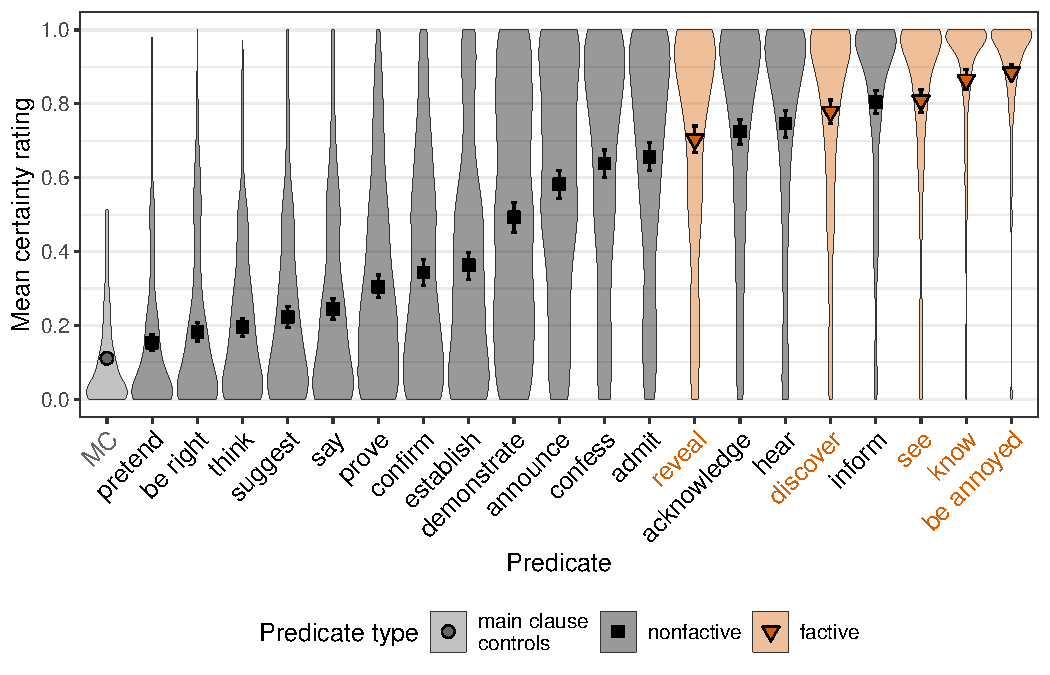
\includegraphics[width=.8\textwidth]{../../../results/main/graphs/mean-certainty-by-predicateType}
\caption{Mean certainty rating (measuring projection) of main clause (`MC') content and the contents of the complements of the 20 \color{orange}factive \color{black} and \color{black}nonfactive \color{black} predicates investigated in Exp.~1a of \citealt{degen-tonhauser-language}. Error bars indicate 95\% bootstrapped confidence intervals. Violin plots indicate the kernel probability density of the individual participants' ratings.}\label{fig:dt1a}
\end{figure}

An alternative proposal for how to distinguish presuppositional projection inferences from nonpresuppositional ones was made in \citealt{mandelkern-etal2020}.\footnote{How to distinguish presuppositions from nonpresuppositions is not the main research question of \citealt{mandelkern-etal2020}. Rather, this paper is primarily concerned with the question of whether presupposition filtering is symmetric.} Specifically, they proposed (p.497) that ``comparing contexts which support the inference to contexts in which it has been made clear that the speaker is ignorant about the inference provides a way to distinguish a broad class of natural and invited pragmatic inferences from those that are really encoded as presuppositions''. For example, on this proposal, the presupposition contributed by \emph{stop} in (\ref{mtrig}c) is expected to receive relatively higher naturalness ratings in the support context in (\ref{mtrig}b) than in the explicit ignorance context in (\ref{mtrig}a). On the other hand, the naturalness ratings for the nonpresupposition contributed by \emph{now frowns on} in (\ref{mtrig}c) are not expected to vary by context. What this measure is taken to distinguish, thus, are projection inferences that are merely ``natural and invited pragmatic inferences'' and projection inferences that are ``encoded as presuppositions, and thus have no choice but to project'' (\citealt[497]{mandelkern-etal2020})

\begin{exe}
\ex\label{mtrig} \citealt[490f.]{mandelkern-etal2020}
\begin{xlist}
\ex Explicit ignorance context: \\ Mary always was involved in a lot of sports, but I don't know whether she ever did any yoga.
\ex Support context: \\ Mary always was involved in a lot of sports, and she used to do yoga, too.
\ex Sentence with presupposition / nonpresupposition: \\ If Mary \{has stopped / now frowns on\} doing yoga, then Matthew will interview her for his story.
\end{xlist}
\end{exe}

The data reported on in \citealt[Exp.~3]{mandelkern-etal2020} supports their proposal, as shown in panel (a) of Fig.~\ref{fig:both-contexts}.\footnote{The data from \citealt[Exp.~3]{mandelkern-etal2020} are available at \url{https://osf.io/2b9m7/}. The R script that generates the figures in panel (a) of Fig.~\ref{fig:both-contexts} and panel (a) of Fig.\ref{fig:eic} is in \url{NEED TO FILL IN LINK AT THE END}.} This figure shows the mean naturalness ratings, by context, of the four supposed presuppositions and four supposed nonpresuppositions featured in their Exp.~3 in sentences like those in (\ref{mtrig}c). As shown, the ratings for \emph{continue, be happy, stop} and \emph{be aware} (in \colorbox{orange}{\color{white}orange\color{black}}) are higher in the support context than in the explicit ignorance context, whereas the ratings for \emph{now frown on, be sure, be hoping} and \emph{enjoy} (in \colorbox{black}{\color{white}black\color{black}}) do not exhibit by-context variation. For \citealt{mandelkern-etal2020}, these results support the assumption that the projection inferences associated with \emph{continue, be happy, stop} and \emph{be aware} are presuppositions, while those of \emph{now frown on, be sure, be hoping} and \emph{enjoy} are not.

However, data reported on in \citealt{kalomoiros-schwarz2024} does not support \citepos{mandelkern-etal2020} proposal as clearly.\footnote{As with \citealt{mandelkern-etal2020}, the distinction between presuppositions and nonpresuppositions was not the main research question of \citealt{kalomoiros-schwarz2024}, but rather the question of whether presupposition filtering is symmetric.} Panels (b) and (c) of Fig.~\ref{fig:both-contexts} show the mean naturalness ratings, by context, of the expressions featured in their Exps.~1 and 2, respectively.\footnote{The data from \citealt{kalomoiros-schwarz2024} are available at \url{https://osf.io/3p68r/}. The R script that generates the figure in panels (b) and (c) of Fig.~\ref{fig:both-contexts} and panel (b) and (c) of Fig.\ref{fig:eic} is in \url{NEED TO FILL IN LINK AT THE END}.} (These experiments did not include nonpresuppositional projection inferences.) As shown in panel (b), the supposed presuppositions of \emph{again, continue} and \emph{find out} appear to be sensitive to the context manipulation, but those of \emph{be aware, stop} and \emph{be happy} do not, contrary to expectation. As shown in panel (c), the relevant data from their Exp.~2 do support \citepos{mandelkern-etal2020} proposal for the supposed presuppositions of \emph{continue, again} and \emph{stop}. The experiments in \citealt{mandelkern-etal2020} and \citealt{kalomoiros-schwarz2024} differed on a number of dimensions, including whether nonpresuppositional projection inferences were included, the number and type of presuppositional projection inferences investigated, and whether the target stimuli investigated presupposition filtering in conjunctions and disjunctions, or only in conjunctions. It is an open question which factors are responsible for the differences in the results for sentences like (\ref{mtrig}c). It is therefore also an open question whether comparison of naturalness ratings in explicit ignorance and support contexts distinguishes presuppositional projection inferences from nonpresuppositional ones, as proposed in \citealt{mandelkern-etal2020}.

\begin{figure}[h!]
\centering
\begin{subfigure}{1\textwidth}
\centering
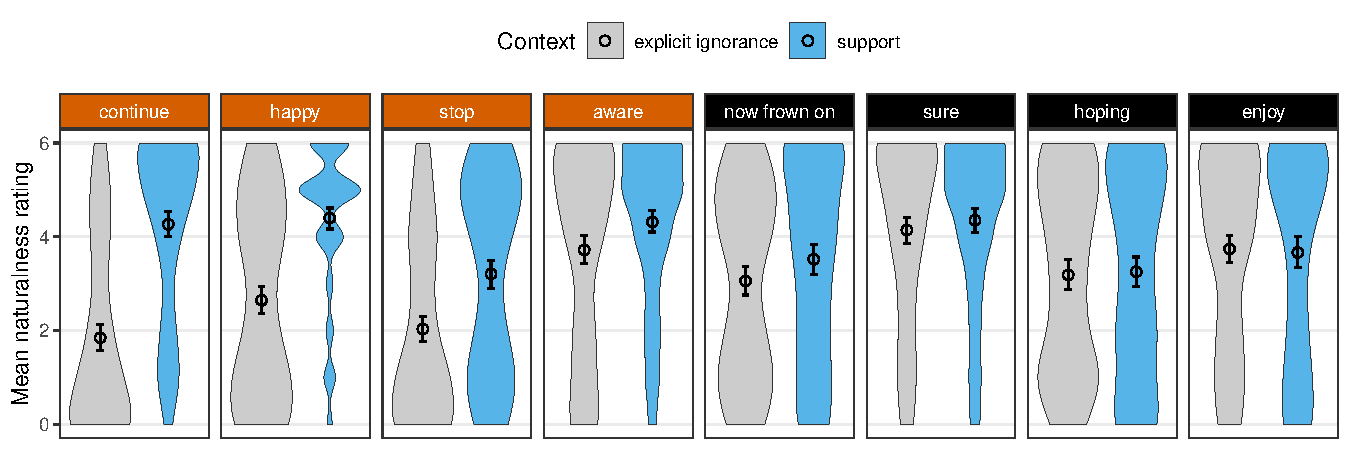
\includegraphics[width=.9\textwidth]{../../../mandelkern-etal2020/graphs/naturalness-by-context-and-expression}
\caption{\citealt[Exp.~3]{mandelkern-etal2020}}
\end{subfigure}

\begin{subfigure}{1\textwidth}
\centering
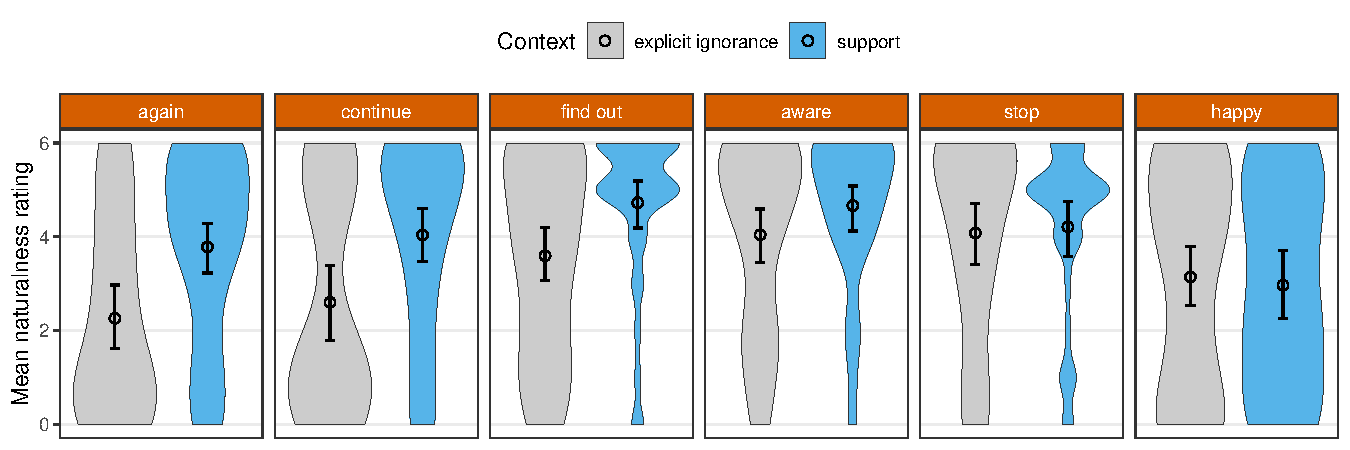
\includegraphics[width=.9\textwidth]{../../../kalomoiros-schwarz2024/exp1/graphs/naturalness-by-context-and-expression} 
\caption{\citealt[Exp.~1]{kalomoiros-schwarz2024}}
\end{subfigure}

\begin{subfigure}{1\textwidth}
\centering
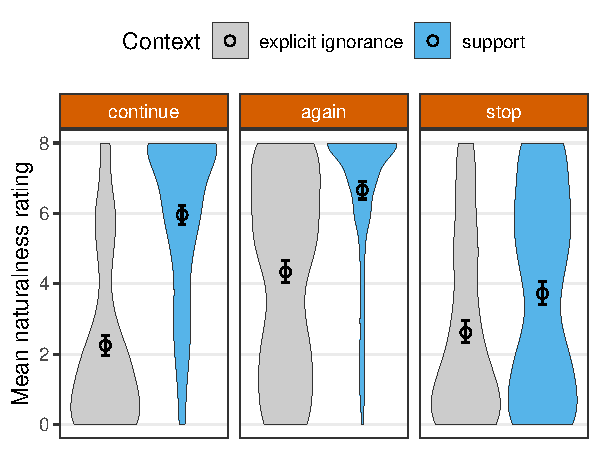
\includegraphics[width=.37\textwidth]{../../../kalomoiros-schwarz2024/exp2/graphs/naturalness-by-context-and-expression}
\caption{\citealt[Exp.~2]{kalomoiros-schwarz2024}}
\end{subfigure}

\caption{Mean naturalness rating in explicit ignorance and support contexts for the (a)  eight presumed presuppositions and nonpresuppositions investigated in \citealt[Exp.~3]{mandelkern-etal2020}, (b) six presumed presuppositions investigated in \citealt[Exp.~1]{kalomoiros-schwarz2024}, and (c) three presumed presuppositions investigated in \citealt[Exp.~2]{kalomoiros-schwarz2024}. Presumed presuppositions given in orange, presumed nonpresuppositions in black. Expressions associated with the (non)presuppositions ordered from left to right by decreasing difference between naturalness rating means in the two contexts. Error bars indicate 95\% bootstrapped confidence intervals. Violin plots indicate the kernel probability density of the individual participants' ratings.}\label{fig:both-contexts}
\end{figure}

This paper presents the results of an experiment designed to investigate \citepos{mandelkern-etal2020} proposal that comparison of naturalness ratings in explicit ignorance and support contexts distinguishes presuppositional from nonpresuppositional projection inferences.\footnote{\label{f:github}The experiment was approved by the ethics review committee of [university name suppressed]. The experiment, materials, data, and analysis scripts can be accessed here:  \url{https://anonymous.4open.science/r/naturalness-in-EIC-5847}.}  To allow for comparison with the results of \citealt{degen-tonhauser-language}, the contents of the complements of the same 20 (non)factive clause-embedding predicates (see Fig.~\ref{fig:dt1a}) were investigated. Our experiment slightly deviated from design of \citepos{mandelkern-etal2020} Exp.~3  to also allow for comparison with the result of \citealt{degen-tonhauser-openmind} that projection is sensitive to prior probability. Specifically, what \citealt{degen-tonhauser-openmind} found was that the higher the prior probability of a content, the stronger the projection inference. For instance, a speaker's commitment to the CC of (\ref{prior}c), that Julian dances salsa, was stronger in the context in (\ref{prior}b), where the CC has a higher prior probability, than in the context in (\ref{prior}a), where the CC has a lower prior probability.

\begin{exe}
\ex\label{prior}
\begin{xlist}
\ex Julian is German. \hfill [lower prior probability]
\ex Julian is Cuban. \hfill [higher prior probability]
\ex Did Cole discover that Julian dances salsa?
\end{xlist}
\end{exe}
Our experiment replaced \citepos{mandelkern-etal2020} support context (which entailed the relevant content) with two support contexts that differed in the prior probability of the CC, namely a lower and a higher prior probability context.\footnote{Another change was that participants gave their naturalness ratings on a slider with endpoints labeled `totally unnatural' and `totally natural' rather than on a 7-point Likert scale with endpoints labeled `completely unnatural' and `completely natural' (as in \citealt[Exp.3]{mandelkern-etal2020} and \citealt[Exp.~1]{kalomoiros-schwarz2024}) or on a 9-point Likert scale with the aforementioned endpoints (\citealt[Exp.~2]{kalomoiros-schwarz2024}).} % Under analyses of presuppositions like \citealt{heim83} or \citealt{vds92}, presuppositions are by default globally accommodated in contexts that are compatible with the presupposition, like these lower and higher prior probability contexts. Accordingly, such analyses predict that presuppositions are rated as natural in lower and higher probability contexts, just as in \citepos{mandelkern-etal2020} entailing support context.

Our experiment also included nontarget stimuli with \emph{stop, continue, again, too, also} and an {\em it}-cleft, which were presented only in explicit ignorance contexts. The inclusion of these stimuli was motivated by the fact that some research on presuppositions assumes that presuppositions exhibit variation in their acceptability in explicit ignorance contexts. Specifically, \citealt{simons01} and \citealt{abusch10} assumed that acceptability in explicit ignorance contexts distinguishes nondefeasible (or: hard) presuppositions from defeasible (or: soft) ones. For instance, the presuppositions associated with \emph{stop}, \emph{discover} and \emph{win} were assumed to be defeasible because they were judged to be acceptable in explicit ignorance contexts, as shown in (\ref{eic2}a-c), respectively. By contrast, the presuppositions associated with \emph{again}, the \emph{it}-cleft and \emph{too} were assumed to be nondefeasible because they were judged to be unacceptable in explicit ignorance contexts, as shown in (\ref{eic3}a-c).

\begin{exe}
\ex\label{eic2}
\begin{xlist}
\ex I have no idea whether Jane ever smoked, but she hasn't stopped smoking. \hfill (\citealt[443]{simons01})
\ex Context: ``two people [\ldots] know that Henry is searching for Jane, but who don't themselves know where Jane is:'' \\ If Henry discovers that Jane is in New York, there'll be trouble. \hfill (\citealt[434]{simons01})
\ex I have no idea whether John ended up participating in the
Road Race yesterday. But if he won it, then he has more victories than anyone else in history. \hfill (\citealt[39]{abusch10})
\end{xlist}
\ex\label{eic3}
\begin{xlist}
\ex\infelic I don't know if Jane ever rented ``Manhattan'' before, but perhaps she's renting it again. \hfill (\citealt[443]{simons01})

\ex \verymarginal I have no idea whether anyone read that letter. But if it is John
who read it, let's ask him to be discreet about the content. \hfill (\citealt[40]{abusch10})

\ex \verymarginal I have no idea whether John read that proposal. But if Bill read it too, let's ask them to confer and simply give us a yes-no response. \hfill (\citealt[40]{abusch10})
\end{xlist}
\end{exe}

Panels (a) to (c) of Fig.~\ref{fig:eic} plots the mean naturalness ratings of the (non)presuppositions investigated in \citealt[Exp.~3]{mandelkern-etal2020}, and Exps.~1 and 2 of \citealt{kalomoiros-schwarz2024}. As shown, the results of these experiments support the assumption of \citealt{simons01} and \citealt{abusch10} that presuppositions vary in their acceptability in explicit ignorance contexts. Furthermore, some of the results agree with the empirical claims of \citealt{simons01} and \citealt{abusch10}. For instance, the mean naturalness rating of \emph{again} is quite low in \citepos{kalomoiros-schwarz2024} Exp.~1 in panel (b), while that of \emph{stop} is quite high, in line with \citepos{abusch10} claim that the presupposition of \emph{again} is nondefeasible and \citepos{simons01} claim that the presupposition of \emph{stop} is defeasible. The results of \citepos{kalomoiros-schwarz2024} Exp.~2 in panel (c), however, show the opposite pattern for \emph{stop} and \emph{again}. It therefore remains an open question whether naturalness ratings of supposed presuppositions in explicit ignorance contexts distinguish nondefeasible and defeasible presuppositions.\footnote{\citealt[734ff.]{roberts-simons2024} suggested that \emph{continue}, unlike \emph{stop}, contributes an anaphoric contextual requirement. This hypothesis goes well with the observation that the naturalness ratings for \emph{continue} are very low across all of the data shown in Fig.~\ref{fig:eic}.}

\begin{figure}[h!]
\centering
\begin{subfigure}{1\textwidth}
\centering
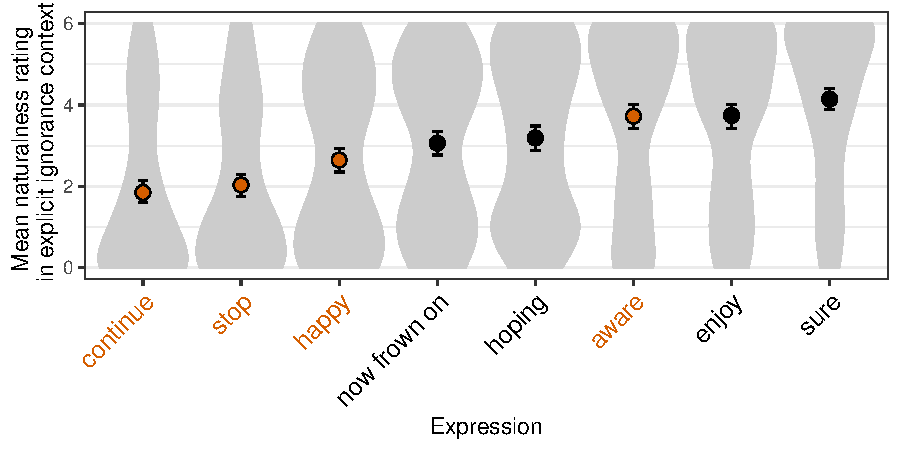
\includegraphics[width=.65\textwidth]{../../../mandelkern-etal2020/graphs/explicit-ignorance-naturalness-by-expression}
\caption{\citealt[Exp.~3]{mandelkern-etal2020}}
\end{subfigure}

\begin{subfigure}{.64\textwidth}
\centering
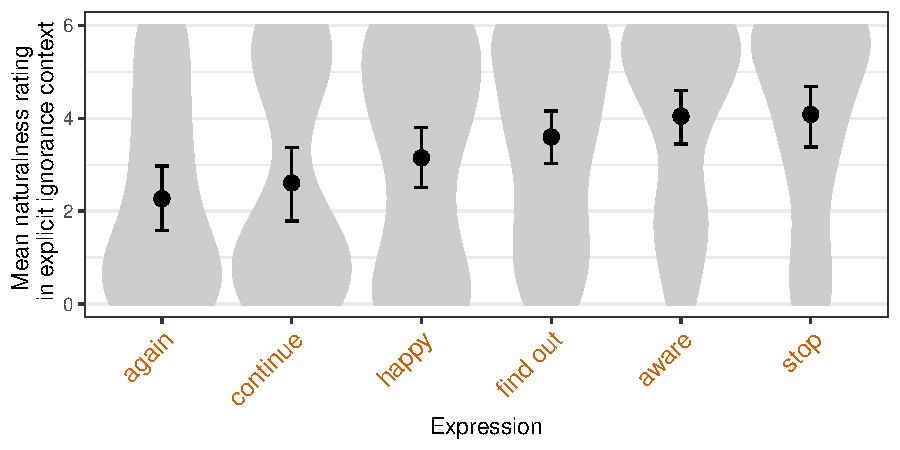
\includegraphics[width=1\textwidth]{../../../kalomoiros-schwarz2024/exp1/graphs/explicit-ignorance-naturalness-by-expression}
\caption{\citealt[Exp.~1]{kalomoiros-schwarz2024}}
\end{subfigure} \begin{subfigure}{.35\textwidth}
\centering
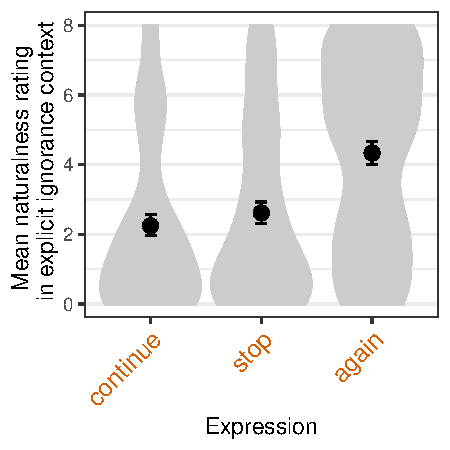
\includegraphics[width=.9\textwidth]{../../../kalomoiros-schwarz2024/exp2/graphs/explicit-ignorance-naturalness-by-expression}
\caption{\citealt[Exp.~2]{kalomoiros-schwarz2024}}
\end{subfigure} 

\caption{Mean naturalness rating in explicit ignorance for the (a)  eight presumed presuppositions and nonpresuppositions investigated in \citealt[Exp.~3]{mandelkern-etal2020}, (b) six presumed presuppositions investigated in \citealt[Exp.~1]{kalomoiros-schwarz2024}, and (c) three presumed presuppositions investigated in \citealt[Exp.2]{kalomoiros-schwarz2024}. Presumed presuppositions given in orange, nonpresuppositions in black. Error bars indicate 95\% bootstrapped confidence intervals. Expressions ordered from left to right by increasing mean naturalness rating. Violin plots indicate the kernel probability density of the individual participants' ratings.}\label{fig:eic}
\end{figure}

\section{Experiment}\label{s2}

To investigate \citepos{mandelkern-etal2020} proposal that comparison of naturalness ratings in explicit ignorance and support contexts distinguishes presuppositional projection inferences from nonpresuppositional ones, participants read two-sentence discourses consisting of a declarative (which provided the context) and an interrogative (which realized a factive or nonfactive predicate), and rated the naturalness of the interrogative in the context of the declarative.

\subsection{Methods}\label{s-methods}

\subsubsection{Participants}

We recruited 425 participants on Prolific. Due to a programming error, the data of only 398 participants was recorded (ages: 19-73, mean: 40.8; 187 women, 201 men, 8 non-categorical, 2 preferred to not disclose). The recruited participants were required to live in the USA, to speak English as their first language, to have completed at least 100 tasks, and to have an approval rating of at least 99\%. The median time spent on the task was 6:24 minutes. Participants were paid \$1.78, corresponding to an hourly pay of \$16.6.


\subsubsection{Materials}

Participants read two-sentence discourses consisting of a declarative followed by an interrogative, as shown in (\ref{sample}). In the target stimuli, the interrogatives combined the 20 (non)factive predicates of \citealt{degen-tonhauser-language} (see Fig.~\ref{fig:dt1a}) with the 20 complement clauses of \citealt{degen-tonhauser-language}, for a total of 400 interrogatives. The preceding declaratives implemented a three-level context condition: In the `explicit ignorance' context (\ref{sample}a), the declarative sentence conveyed the speaker's ignorance about the CC. In the `lower prior probability' context (\ref{sample}b), the CC had a comparatively lower prior probability, whereas it had a comparatively higher prior probability in the `higher prior probability' context (\ref{sample}c). The two contexts for each of the 20 complement clauses were normed in \citealt{degen-tonhauser-openmind}. See Supplement \ref{a:clauses} for the full set of 20 complement clauses and the two contexts for each complement clause.

\begin{exe}
\ex\label{sample}
\begin{xlist}
\ex Explicit ignorance context: \\ I have no idea if Julian dances salsa. Did Cole discover that Julian dances salsa?
\ex Lower prior probability context: \\ Julian is German. Did Cole discover that Julian dances salsa?
\ex Higher prior probability context: \\ Julian is Cuban. Did Cole discover that Julian dances salsa?'
\end{xlist}
\end{exe}

In addition to the 1,200 target stimuli (400 interrogatives $\times$ 3 contexts), the materials also included the six nontarget stimuli in (\ref{filler}). The interrogatives of these stimuli featured six expressions typically analyzed as presupposition triggers, namely {\em stop, continue, again, too, also}, and an {\em it-}cleft. The preceding declaratives conveyed the speaker's explicit ignorance about presuppositions associated with these expressions, namely the pre-state contents of \emph{stop} and \emph{continue}, the prejacent of \emph{again}, the content that there is an alternative true proposition of \emph{too} and \emph{also}, and the existential content of the \emph{it}-cleft.\footnote{The contents investigated for {\em too} and {\em also} in (\ref{filler}d) and (\ref{filler}e) are that Ann plays an instrument other than the flute and that Svenja plays a sport other than soccer. This interpretation arises if {\em too} and {\em also} associate with {\em the flute} and {\em soccer}, respectively. While prosody was not controlled for, this focus association is made plausible by the preceding explicit ignorance statements, which evoke the question of whether Ann plays any instrument and whether Svenja plays any sport, respectively.}  As noted in \S1, \citealt{simons01} took {\em stop} to be a soft trigger and \emph{again} a hard trigger; \citealt{abusch10} assumed that \emph{too} and \emph{it}-clefts are hard triggers. The nontarget stimuli were included for comparison to the target stimuli, to the claims of \citealt{simons01} and \citealt{abusch10}, and to the results of \citealt[Exp.~3]{mandelkern-etal2020} and \citealt[Exps.~1-2]{kalomoiros-schwarz2024}, where  \emph{continue, stop} and \emph{again} were target expressions. 

%\citealt{kalomoiros-schwarz2021}: (continue, again, aware, find out, happy, stop)
%\citealt{kalomoiros-schwarz2024}:  (continue,again,aware,find out,happy,stop),

\begin{exe}
\ex\label{filler} 
\begin{xlist}
\ex I don't know if Stephen was ever in the habit of vaping. Has Stephen recently stopped vaping?
\ex I don't know if John was ever reading ``Dune''. Has John recently continued reading ``Dune''?
\ex I don't know if William was ever interested in history. Is William interested in history again?"
\ex I don't know if Ann plays any instrument. Does Ann play the flute, too?
\ex I don't know if Svenja plays any sport. Does Svenja also play soccer?
\ex I don't know if anyone was playing outside with the kids. Was it Jack who was playing outside with the kids?

\end{xlist}
\end{exe}

The experiment also included 4 filler stimuli that were used to exclude the data of participants not attending to the task (see Supplement \ref{a:fillerPractice}). The filler stimuli, which also consisted of a declarative followed by an interrogative, were expected to receive high naturalness ratings.

A random set of 30 stimuli was created for each participant. Each set contained 20 target stimuli in which each of the 20 complement clauses was paired with a unique clause-embedding predicate. Twelve of the target stimuli were presented in the explicit ignorance context, and the other eight in a low or a higher prior probability context (four each). Each participants' set also contained the same six nontarget stimuli and the same four filler stimuli. Each of the 30 stimuli were presented as utterances by a unique named speaker. Trial order was randomized for each participant. 

\subsubsection{Procedure}

Participants were instructed to rate how natural the question sounds in the context of the statement. As shown in Figure \ref{f:trials}, they were asked give their rating on a slider from `totally unnatural' (coded as 0) to `totally natural' (coded as 1). The experiment began with four practice trials to familiarize participants with the task (see Supplement \ref{a:fillerPractice} for details). After rating the 30 trials, participants filled out a short optional demographic survey. To encourage truthful responses, participants were told that they would be paid no matter what answers they gave in the survey.


\begin{figure}[h]
\centering
%\begin{subfigure}{0.49\textwidth}
\fbox{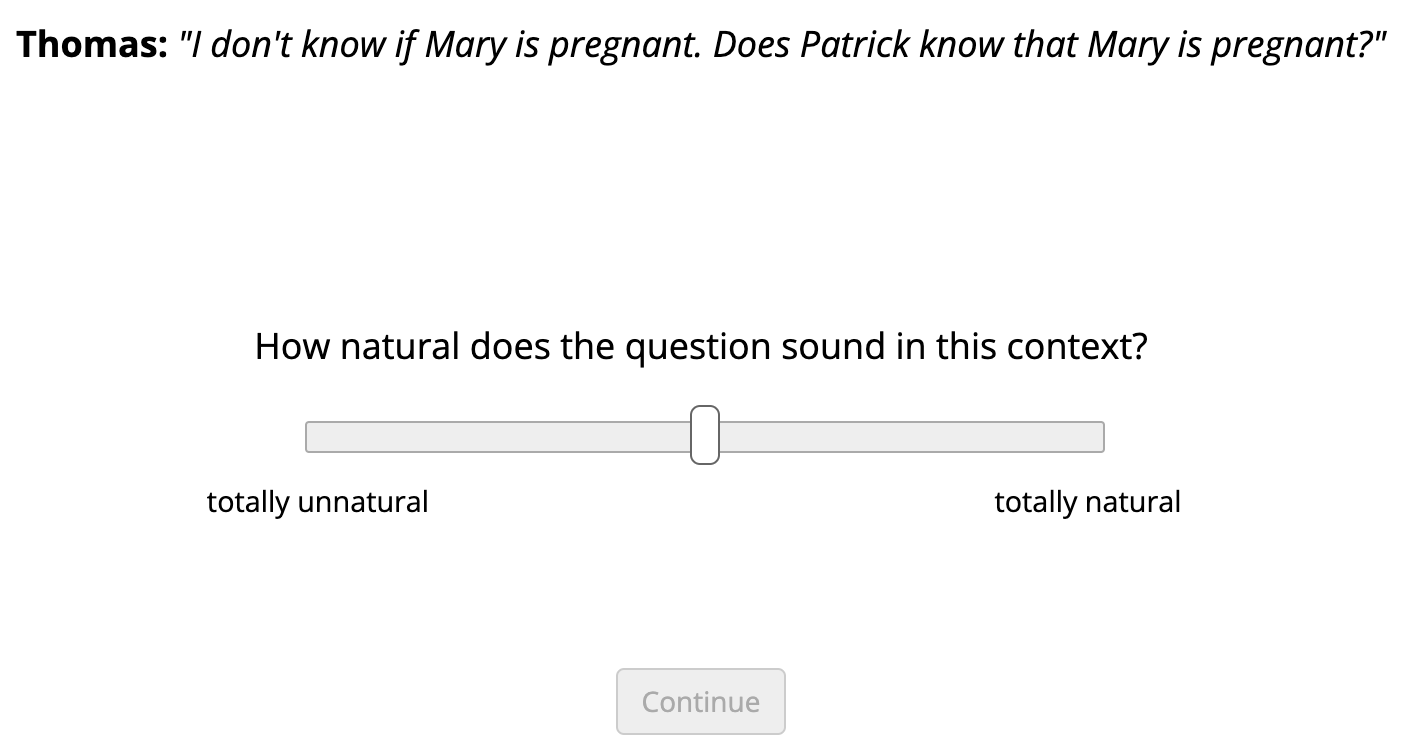
\includegraphics[width=.7\textwidth]{figures/trial-eic}}
%\caption{Trial with explicit ignorance context}
%\end{subfigure}
%\\[.1cm]
%\begin{subfigure}{0.49\textwidth}
%\fbox{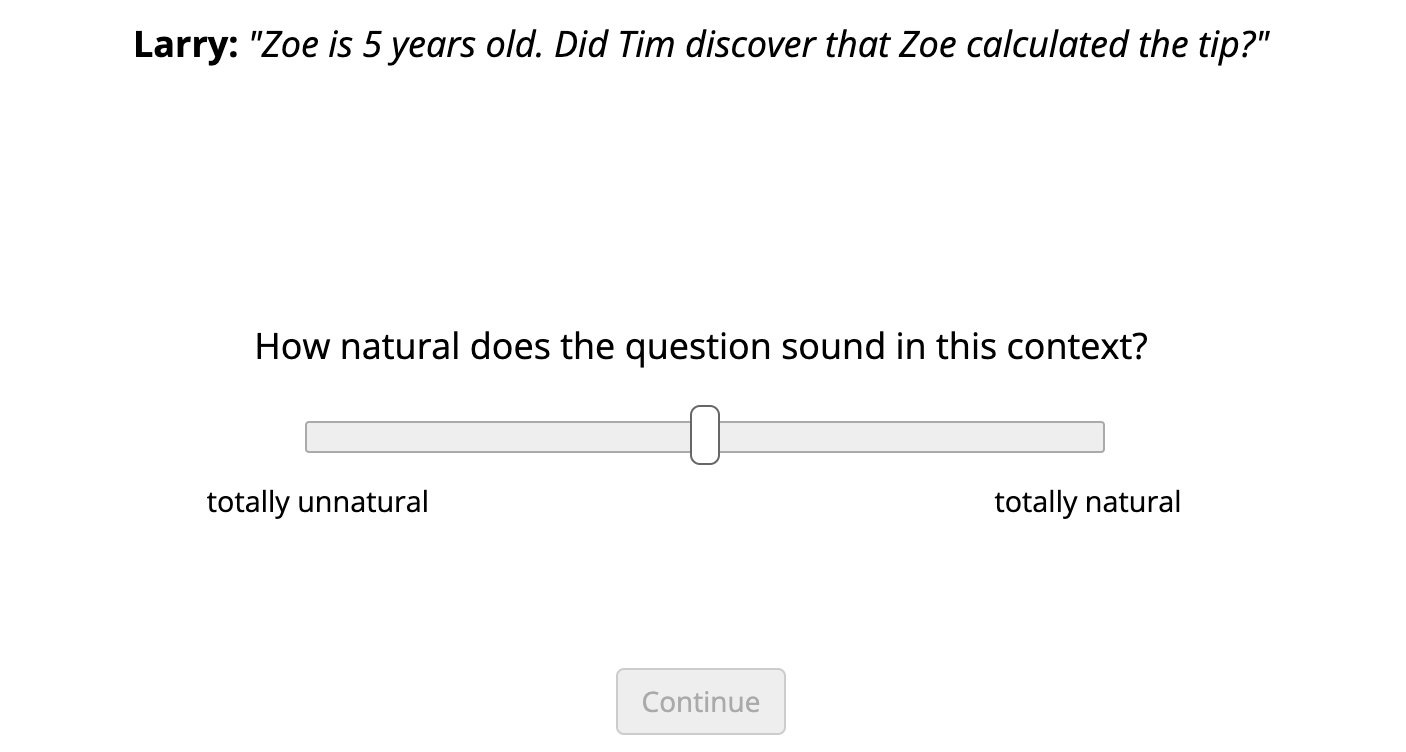
\includegraphics[width=\textwidth]{figures/trial-low}}
%\caption{Trial with lower prior probability context}
%\end{subfigure} \hfill \begin{subfigure}{0.49\textwidth}
%\fbox{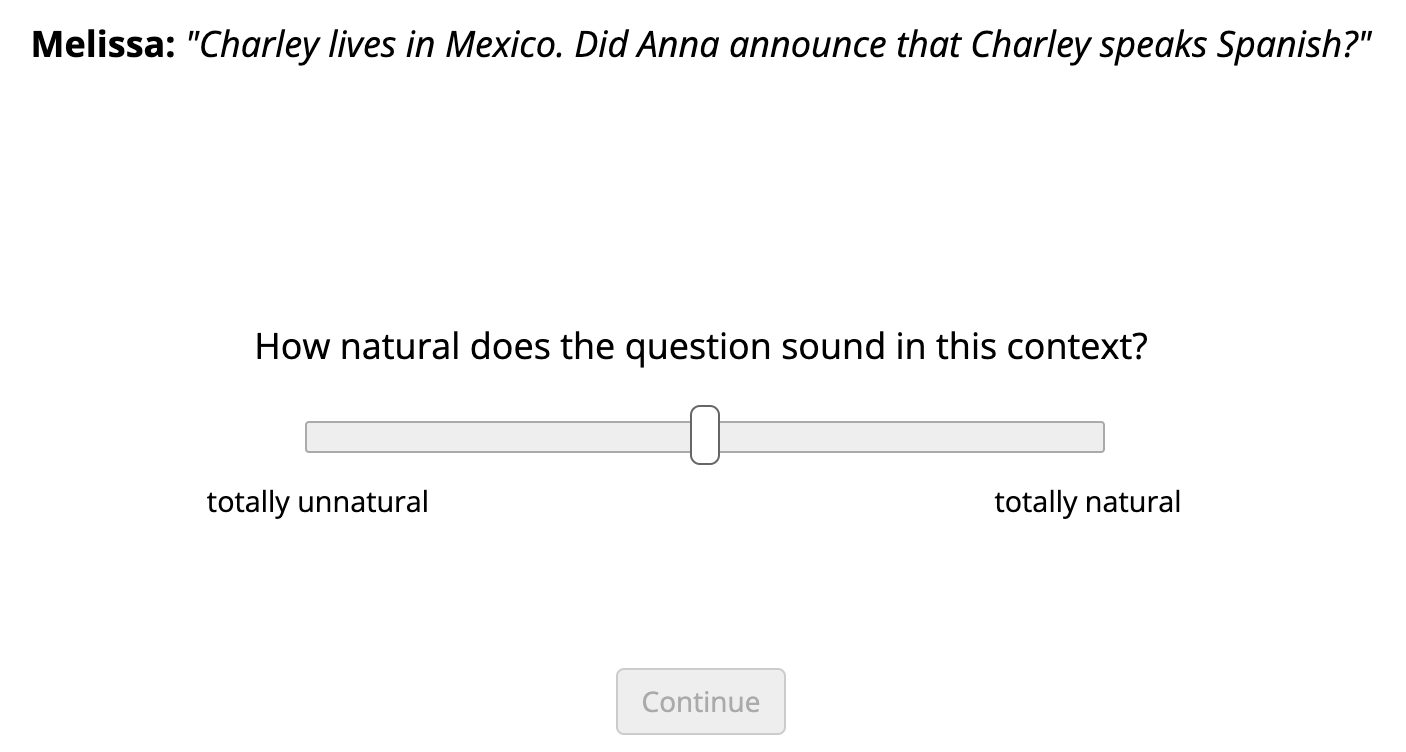
\includegraphics[width=\textwidth]{figures/trial-high}}
%\caption{Trial with higher prior probability context}
%\end{subfigure}
\caption{Sample trial with explicit ignorance context.}\label{f:trials}
\end{figure}


\subsubsection{Data exclusion} 

We excluded the data of 5 participants who did not self-identify as native speakers of American English and that of 23 participants whose mean response to the fillers (expected to be natural) was more than 2 sd below the group mean.\footnote{Contrary to what was planned, one of the four filler stimuli was not used to exclude participants' data because it had a mean rating of only .5. See Supplement \ref{a:fillerPractice} for details.} The data of 370 participants entered into the analysis (ages: 19-80, mean: 40.7; 175 women, 185 men, 8 nonbinary, 2 did not disclose). The 20 predicates each received at least 200 ratings in the explicit ignorance context (mean: 222 ratings), at least 59 ratings in the lower prior probability context (mean: 74), and at least 61 ratings in the higher prior probability context (mean: 74). The six nontargets received 370 ratings each. 

\subsection{Results}

We first investigate \citepos{mandelkern-etal2020} proposal that comparison of naturalness ratings in explicit ignorance and support contexts distinguishes presuppositional projection inferences from nonpresuppositional ones (\S\ref{s:analysis2}). We then address the question of how projection inferences behave in explicit ignorance contexts and, specifically, whether naturalness ratings in such contexts distinguish nondefeasible and defeasible presuppositions, as proposed in \citealt{simons01} and \citealt{abusch10} (\S\ref{s:analysis1}).

\subsubsection{Comparison of naturalness ratings in explicit ignorance and support contexts}\label{s:analysis2}

Does comparison of naturalness ratings of in explicit ignorance and support contexts distinguish between presuppositional projection inferences and nonpresuppositional ones, as proposed in \citealt{mandelkern-etal2020}? Fig.~\ref{fig:acc-by-context} shows mean naturalness ratings for the CCs of the 20 \fcolorbox{black}{orange}{\color{white}factive\color{black}} and \fcolorbox{black}{black}{\color{white}nonfactive\color{black}} predicates in the three contexts featured in our experiment with predicates ordered left-to-right (and top-to-bottom) by decreasing difference in the ratings in the higher prior probability and explicit ignorance contexts. The figure also includes the results of the statistical analysis, namely posthoc pairwise comparisons of the estimated means for each context using the `emmeans' package (\citealt{emmeans}); a separate comparison was conducted for each of the 20 predicates. The input to the pairwise comparisons were 20 Bayesian mixed-effects beta regression models with weakly informative priors that were fit using the `brms' package (\citealt{buerkner2017}). The models predicted  naturalness ratings\footnote{\label{fn:transform}To model the ratings using a beta regression, the ratings were first transformed from the interval [0,1] to the interval (0,1) using the method proposed in \citealt{smithson-verkuilen2006}.} from a fixed effect of context (with treatment coding and `explicit ignorance' as reference level) and included a random by-item intercept (where an item is a complement clause) and a random by-item slope for context.\footnote{By-participant random effects were not included because each participant saw each predicate only once and in only one context condition.} The output of the pairwise comparison for each expression was the 95\% HDI of estimated marginal mean differences between each of the three contexts. We assume that two contexts differ if their HDI does not include 0. In Fig.~\ref{fig:acc-by-context}, a solid line spanning two contexts indicates that the ratings in the two contexts differ.\footnote{The full model output is available here: \url{https://anonymous.4open.science/r/naturalness-in-EIC-5847/results/main/models/analysis2/fullModelOutput/fullModelOutput.pdf}.} 

As shown, the effect of context is not uniform for the projection inferences of the purported factive predicates. For {\em be annoyed, know} and {\em discover}, the mean naturalness rating is lower in the explicit ignorance context than in the higher prior probability context, but this is not the case for {\em see} and {\em reveal}, which pattern like several nonfactive predicates in this regard. Thus, on \citepos{mandelkern-etal2020} proposal, only inferences to the contents of the complements of \emph{be annoyed, know} and \emph{discover} would be considered presuppositional projection inferences; these three predicates, which include an emotive predicate, a cognitive stative predicate, and a cognitive change-of-state predicate, do not necessarily constitute a natural class (see, e.g., \citealt{karttunen2016,djaerv-thesis}). Inferences to the contents of the complements of \emph{see} and \emph{reveal} would be considered nonpresuppositional projection inferences, like those to the contents of the complements of communication predicates like \emph{inform} and \emph{announce} (for discussion, see \citealt{anand-hacquard2014}).\footnote{Our five purportedly factive predicates received ratings in the higher prior probability support context that are roughly comparable to the ratings that the factive predicates of \citealt{mandelkern-etal2020} received in the support context. Specifically, the mean naturalness ratings in the higher prior probability support context ranged from .64 ({\em reveal}) to .78 ({\em know}) on a scale from 0 to 1; the mean naturalness ratings in the support context of \citealt{mandelkern-etal2020} were 4.32  for {\em be aware} and 4.4 for {\em be happy} on a scale from 1 to 7.} Alternatively, the results suggest that comparison of naturalness ratings in explicit ignorance and support contexts does not reliably distinguish presuppositional projection inferences from nonpresuppositional ones. Importantly, the difference between the higher prior probability and explicit ignorance contexts for \emph{be annoyed} and \emph{know} are driven primarily by the low naturalness ratings in the explicit ignorance contexts, a point we return to in \S\ref{s:discussion}.


We also observe that the prior probability of content modulates naturalness ratings with all predicates, except {\em confess, demonstrate, pretend} and {\em confirm}, such that content is judged as more natural in a context in which it has a higher prior probability than in a context in which it has a lower prior probability. This result dovetails with the result of \citealt{degen-tonhauser-openmind} that projection is modulated by prior probability. Thus, a methodological implication of our experiment is that future investigations of projection inferences using naturalness ratings will need to consider the effect of the prior probability of the inference.

\begin{figure}[h!]
\centering
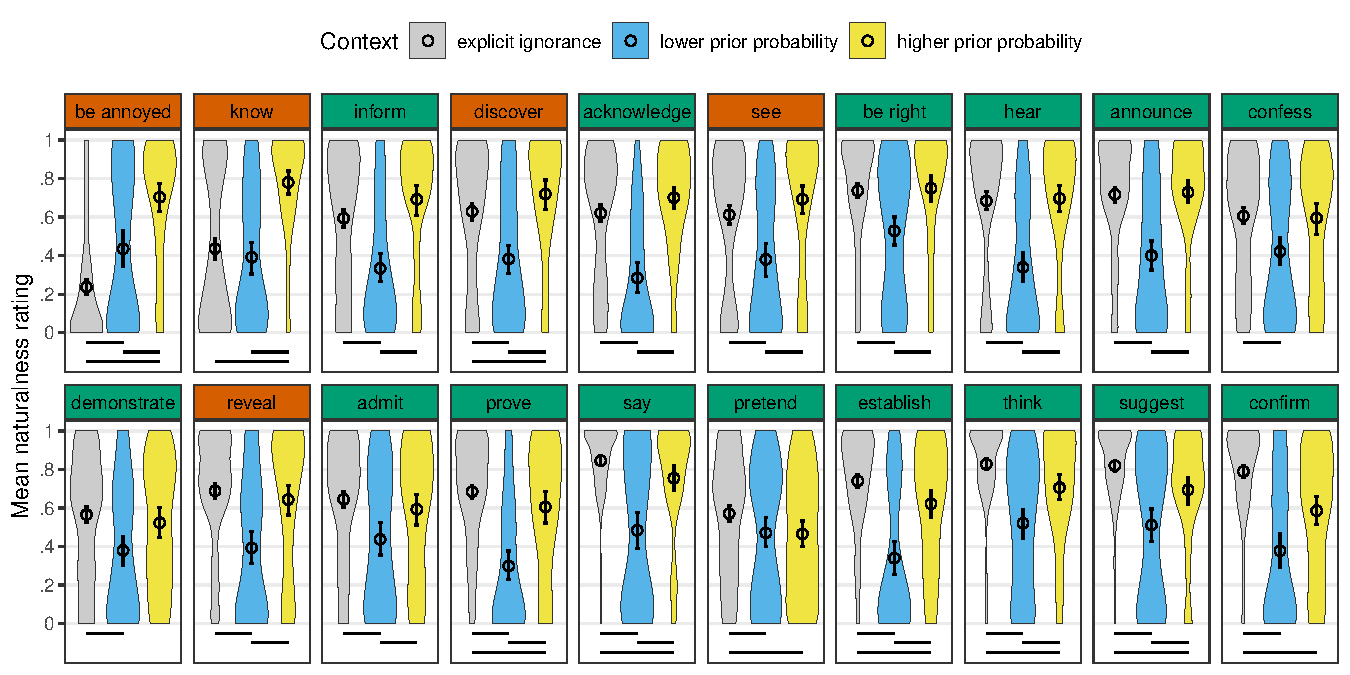
\includegraphics[width=\textwidth]{../../../results/main/graphs/naturalness-by-context-and-predicate-with-stats}
\caption{Mean naturalness rating by predicate (\fcolorbox{black}{orange}{factive}, \fcolorbox{black}{green}{nonfactive}) and context, with predicates ordered from left to right (and top to bottom) by decreasing difference between the mean rating in the higher prior probability support context and the explicit ignorance context. Error bars indicate 95\% bootstrapped CIs. Violin plots indicate kernel probability density of participants' ratings. Below each facet, a solid line spanning two contexts indicates that the 95\% HDI of estimated marginal mean differences between the two contexts does not include 0, that is, that the ratings in the two contexts differ.}\label{fig:acc-by-context}
\end{figure}

%The linetype indicates  whether the difference is at least 1.5 (solid line: ---), below 1.5 but at least 0.5 (dashed line: -- --), or below 0.5 but above 0 (dotted line: \raisebox{1mm}{\ldots}). 

% As shown in Table \ref{t:pairwise2},\footnote{The full model output is available here: \url{LINK TO TABLE IN REPO}.{\bf ADD AFTER FINALIZING SCRIPTS}} the model confirms that the effect of context is not uniform for the five factive predicates: The difference between the naturalness ratings in the higher prior probability context and the explicit ignorance context is larger for {\em be annoyed} than for {\em know}, which in turn is larger than for {\em see} and {\em discover}. For {\em reveal} there is no difference, just like for many nonfactive predicates, such as {\em admit, hear, announce} and {\em be right}. The comparison of the lower prior probability context and the explicit ignorance context reveals a positive difference for {\em be annoyed}, no difference for {\em know} and a negative difference for {\em see, discover}, and {\em reveal}. Finally, there is a positive difference between the higher and lower prior probability context for all 20 predicates except for {\em demonstrate} and {\em pretend}.
% 
%\begin{table}[!h]
%\addtolength{\tabcolsep}{-.19em}
%\centering
%\begin{tabular}{r  cccccccccccccccccccc}
%& \rots{\color{orange}be annoyed\color{black}} & \rots{\color{orange}know\color{black}} & \rots{\color{green}demonstrate\color{black}} & \rots{\color{green}pretend\color{black}} & \rots{\color{green}inform\color{black}} & \rots{\color{green}confess\color{black}} & \rots{\color{orange}see\color{black}} & \rots{\color{green}acknowledge\color{black}} & \rots{\color{orange}discover\color{black}} & \rots{\color{green}admit\color{black}} & \rots{\color{green}hear\color{black}} & \rots{\color{green}prove\color{black}} & \rots{\color{orange}reveal\color{black}} & \rots{\color{green}announce\color{black}} & \rots{\color{green}be right\color{black}} & \rots{\color{green}establish\color{black}} & \rots{\color{green}confirm\color{black}} & \rots{\color{green}suggest\color{black}} & \rots{\color{green}think\color{black}} & \rots{\color{green}say\color{black}} \\
%\hline
% higher prior - EIC & \cellcolor{yellow1} & \cellcolor{yellow2} & \cellcolor{white} & \cellcolor{purple3} & \cellcolor{white} & \cellcolor{white} & \cellcolor{yellow3} & \cellcolor{white} & \cellcolor{yellow3} & \cellcolor{white} & \cellcolor{white} & \cellcolor{purple2} & \cellcolor{white} & \cellcolor{white} & \cellcolor{white} & \cellcolor{purple2} & \cellcolor{purple2} & \cellcolor{purple2} & \cellcolor{purple3} & \cellcolor{purple2} \\ 
  lower prior - EIC & \cellcolor{yellow2} & \cellcolor{white} & \cellcolor{purple2} & \cellcolor{purple2} & \cellcolor{purple2} & \cellcolor{purple2} & \cellcolor{purple2} & \cellcolor{purple2} & \cellcolor{purple2} & \cellcolor{purple2} & \cellcolor{purple2} & \cellcolor{purple1} & \cellcolor{purple2} & \cellcolor{purple2} & \cellcolor{purple2} & \cellcolor{purple1} & \cellcolor{purple2} & \cellcolor{purple2} & \cellcolor{purple2} & \cellcolor{purple2} \\ 
  higher - lower prior & \cellcolor{yellow2} & \cellcolor{yellow2} & \cellcolor{white} & \cellcolor{white} & \cellcolor{yellow2} & \cellcolor{yellow2} & \cellcolor{yellow2} & \cellcolor{yellow1} & \cellcolor{yellow2} & \cellcolor{yellow2} & \cellcolor{yellow2} & \cellcolor{yellow2} & \cellcolor{yellow2} & \cellcolor{yellow2} & \cellcolor{yellow2} & \cellcolor{yellow2} & \cellcolor{yellow2} & \cellcolor{yellow2} & \cellcolor{yellow2} & \cellcolor{yellow2} \\ 
  

%\hline
%\end{tabular}
%\caption{Posterior distribution of estimated marginal means of pairwise differences between the three contexts for each expression, with expressions ordered by mean naturalness rating in explicit ignorance context. `EIC' stands for explicit ignorance context. Color coding indicates whether the difference was positive or negative, and the size of the difference; a white cell means that there was no difference: \\
%Positive difference: \colorbox{yellow1}{\makebox[4em][c]{$>=-1.5$}}, \colorbox{yellow2}{\makebox[4em][c]{($-1.5, -0.5]$}}, \colorbox{yellow3}{\makebox[4em][c]{($-0.5, 0]$}} \\
%Negative difference: \colorbox{purple1}{\makebox[4em][c]{$>=1.5$}}, \colorbox{purple2}{\makebox[4em][c]{($1.5,0.5]$}}, 
%\colorbox{purple3}{\makebox[4em][c]{($0.5, 0]$}} 
%}\label{t:pairwise2}
%\end{table}


\subsubsection{Naturalness ratings of projection inferences in explicit ignorance contexts}\label{s:analysis1}

Recall that \citealt{simons01} and \citealt{abusch10} assumed that presuppositions vary in their acceptability in explicit ignorance contexts and that, specifically, nondefeasible presuppositions are unacceptable in such contexts and defeasible ones  acceptable. Figure \ref{fig:acc-by-expression} shows mean naturalness ratings in the explicit ignorance context by expression (in distinct colors: \color{orange}factive predicates\color{black}, \color{black}nonfactive predicates\color{black}, \color{gray}nontarget\color{black}). Consistent with \citepos{simons01} and \citepos{abusch10} assumption, there is variation in the mean naturalness ratings of the projection inferences investigated. Looking first at the six nontarget stimuli (for which there was only one item each), the naturalness means for \emph{continue, too, also} and \emph{again} are at floor, which would suggest, given \citepos{simons01} and \citepos{abusch10} assumption, that the projection inferences associated with these expressions are not defeasible, that is, hard (see also \citealt[734ff.]{roberts-simons2024} for \emph{continue}). This result is in line with \citepos{simons01} assumption for \emph{again} and \citepos{abusch10} assumption for \emph{too}. Recall, however, from \S1 that in \citealt[Exp.~2]{kalomoiros-schwarz2024} the mean naturalness rating for \emph{again} was much higher than that those of \emph{continue} and \emph{stop}. 

The results for the two items with \emph{stop} and the \emph{it}-cleft are less clear: The mean naturalness ratings are higher than those of \emph{continue, too, also} and \emph{again}, but not as high as for some of the other contents investigated. These results do not support the assumption that naturalness ratings in explicit ignorance contexts categorically distinguish between defeasible (soft) and nondefeasible (hard) projection inferences. 

The results of our experiment further complicate the picture for \emph{stop}, whose presupposition was taken to be defeasible in \citealt{simons01}, but whose mean rating is lower than the mean rating for the \emph{it}-cleft, whose presupposition was taken to be nondefeasible in \citealt{abusch10}.\footnote{\citealt{smith-hall11} also observed that presupposition of the {\em it-}cleft did not pattern like a nondefeasible inference. \citealt{jayez-etal2015} found that French {\em aussi} `too', {\em regretter} `regret' and clefts are not entirely unnatural in explicit ignorance contexts.} Recall from \S1 that the pre-state content of \emph{stop} received quite low naturalness ratings in \citealt[Exp.~3]{mandelkern-etal2020} and \citealt[Exp.~2]{kalomoiros-schwarz2024}, but not in \citealt[Exp.~1]{kalomoiros-schwarz2024}. These observations suggest that it is still an open question of how defeasible the pre-state content of \emph{stop} is (see also \citealt[192f.]{abrusan2016} for considerations along these lines).

\begin{figure}[h!]
\centering
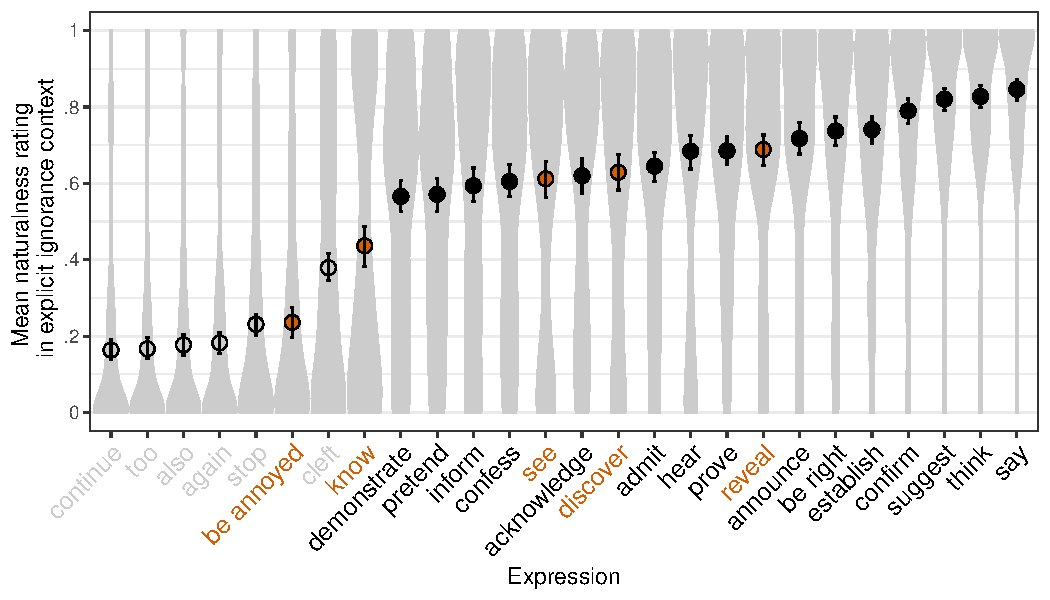
\includegraphics[width=.9\textwidth]{../../../results/main/graphs/explicit-ignorance-naturalness-by-predicate}
\caption{Mean naturalness rating in explicit ignorance context by expression (\color{orange}factive\color{black}, \color{black}nonfactive\color{black}, \color{gray}nontarget\color{black}). Error bars indicate 95\% bootstrapped confidence intervals. Overlaid violin plots indicate the kernel probability density of the participants' ratings.}\label{fig:acc-by-expression}
\end{figure}

The naturalness ratings for the five purportedly factive predicates in explicit ignorance contexts exhibit a heterogeneous pattern, with the mean for \emph{be annoyed} as low as that of \emph{stop}, that of \emph{know} higher but not as high as that of \emph{see, discover} and \emph{reveal}. These means suggest that the projection inferences associated with \emph{see, discover} and \emph{reveal} are defeasible, in line with \citepos{simons01} assumption about \emph{discover}. As already noted in \S\ref{s:analysis2}, the means for \emph{be annoyed} and \emph{know} are quite low, a point we return to in \S\ref{s:discussion}.

These observations were confirmed by a posthoc pairwise comparison of the estimated means for each target and nontarget expression in the explicit ignorance context using the `emmeans' package (\citealt{emmeans}) in R (\citealt{r}). The input to the pairwise comparison was a mixed-effects beta regression model with weakly informative priors that was fit using the `brms' package (\citealt{buerkner2017}). The model predicted naturalness ratings\footnote{As in the model reported in the previous section, the ratings were transformed to the interval (0,1); see footnote \ref{fn:transform}.} from a fixed effect of expression (with treatment coding and `continue' as reference level) and included random by-participant and by-item intercepts (where an item is a complement clause). The output of the pairwise comparison were 95\% highest density intervals (HDIs) of estimated marginal mean differences between each of the expressions. We assume that two expressions differ in their naturalness in the explicit ignorance context if their HDI does not include 0. As shown in Table \ref{t:pairwise},\footnote{While the naturalness ratings collected from the participants range from 0 to 1, the greater than $|$1$|$  estimated marginal mean differences are the result of the beta regression using a logit link function for the mean parameter. The full model output is available here: \url{https://anonymous.4open.science/r/naturalness-in-EIC-5847/results/main/models/analysis1/fullModelOutput/fullModelOutput.pdf}.} the pairwise comparison suggests that the naturalness ratings are lowest for \emph{continue, too, also} and \emph{again}, slightly higher for \emph{stop} and \emph{be annoyed}, slightly higher again for the {\em it-}cleft and \emph{know}, and higher yet again for \emph{see, discover} and \emph{reveal}. Overall, the results suggest that projection inferences vary in how defeasible they are in explicit ignorance contexts, but the observed variation does not suggest a binary, categorical distinction in defeasibility.


\begin{table}[!h]
\addtolength{\tabcolsep}{-.19em}
\centering
\begin{tabular}{r | cccccccccccccccccccccccccc}
& \rots{\bf continue} & \rots{\bf too} & \rots{\bf also} & \rots{\bf again} & \rots{\bf stop} & \rots{\color{orange}{\bf be annoyed}\color{black}} & \rots{\bf cleft} & \rots{\color{orange}{\bf know}\color{black}} & \rots{\color{green}{\bf demonstrate}\color{black}} & \rots{\color{green}{\bf pretend}\color{black}} & \rots{\color{green}{\bf inform}\color{black}} & \rots{\color{green}{\bf confess}\color{black}} & \rots{\color{orange}{\bf see}\color{black}} & \rots{\color{green}{\bf acknowledge}\color{black}} & \rots{\color{orange}{\bf discover}\color{black}} & \rots{\color{green}{\bf admit}\color{black}} & \rots{\color{green}{\bf hear}\color{black}} & \rots{\color{green}{\bf prove}\color{black}} & \rots{\color{orange}{\bf reveal}\color{black}} & \rots{\color{green}{\bf announce}\color{black}} & \rots{\color{green}{\bf be right}\color{black}} & \rots{\color{green}{\bf establish}\color{black}} & \rots{\color{green}{\bf confirm}\color{black}} & \rots{\color{green}{\bf suggest}\color{black}} & \rots{\color{green}{\bf think}\color{black}} & \rots{\color{green}{\bf say}\color{black}} \\
\hline
 {\bf continue} & \cellcolor{black} & \cellcolor{white} & \cellcolor{white} & \cellcolor{white} & \cellcolor{yellow3} & \cellcolor{yellow3} & \cellcolor{yellow2} & \cellcolor{yellow2} & \cellcolor{yellow1} & \cellcolor{yellow1} & \cellcolor{yellow1} & \cellcolor{yellow1} & \cellcolor{yellow1} & \cellcolor{yellow1} & \cellcolor{yellow1} & \cellcolor{yellow1} & \cellcolor{yellow1} & \cellcolor{yellow1} & \cellcolor{yellow1} & \cellcolor{yellow1} & \cellcolor{yellow1} & \cellcolor{yellow1} & \cellcolor{yellow1} & \cellcolor{yellow1} & \cellcolor{yellow1} & \cellcolor{yellow1} \\ 
  {\bf too} & \cellcolor{white} & \cellcolor{black} & \cellcolor{white} & \cellcolor{white} & \cellcolor{yellow3} & \cellcolor{yellow3} & \cellcolor{yellow2} & \cellcolor{yellow2} & \cellcolor{yellow1} & \cellcolor{yellow1} & \cellcolor{yellow1} & \cellcolor{yellow1} & \cellcolor{yellow1} & \cellcolor{yellow1} & \cellcolor{yellow1} & \cellcolor{yellow1} & \cellcolor{yellow1} & \cellcolor{yellow1} & \cellcolor{yellow1} & \cellcolor{yellow1} & \cellcolor{yellow1} & \cellcolor{yellow1} & \cellcolor{yellow1} & \cellcolor{yellow1} & \cellcolor{yellow1} & \cellcolor{yellow1} \\ 
  {\bf also} & \cellcolor{white} & \cellcolor{white} & \cellcolor{black} & \cellcolor{white} & \cellcolor{yellow3} & \cellcolor{yellow3} & \cellcolor{yellow2} & \cellcolor{yellow2} & \cellcolor{yellow2} & \cellcolor{yellow1} & \cellcolor{yellow1} & \cellcolor{yellow1} & \cellcolor{yellow1} & \cellcolor{yellow1} & \cellcolor{yellow1} & \cellcolor{yellow1} & \cellcolor{yellow1} & \cellcolor{yellow1} & \cellcolor{yellow1} & \cellcolor{yellow1} & \cellcolor{yellow1} & \cellcolor{yellow1} & \cellcolor{yellow1} & \cellcolor{yellow1} & \cellcolor{yellow1} & \cellcolor{yellow1} \\ 
  {\bf again} & \cellcolor{white} & \cellcolor{white} & \cellcolor{white} & \cellcolor{black} & \cellcolor{yellow3} & \cellcolor{white} & \cellcolor{yellow2} & \cellcolor{yellow2} & \cellcolor{yellow2} & \cellcolor{yellow2} & \cellcolor{yellow2} & \cellcolor{yellow1} & \cellcolor{yellow1} & \cellcolor{yellow1} & \cellcolor{yellow1} & \cellcolor{yellow1} & \cellcolor{yellow1} & \cellcolor{yellow1} & \cellcolor{yellow1} & \cellcolor{yellow1} & \cellcolor{yellow1} & \cellcolor{yellow1} & \cellcolor{yellow1} & \cellcolor{yellow1} & \cellcolor{yellow1} & \cellcolor{yellow1} \\ 
  {\bf stop} & \cellcolor{purple3} & \cellcolor{purple3} & \cellcolor{purple3} & \cellcolor{purple3} & \cellcolor{black} & \cellcolor{white} & \cellcolor{yellow2} & \cellcolor{yellow2} & \cellcolor{yellow2} & \cellcolor{yellow2} & \cellcolor{yellow2} & \cellcolor{yellow2} & \cellcolor{yellow2} & \cellcolor{yellow2} & \cellcolor{yellow2} & \cellcolor{yellow2} & \cellcolor{yellow1} & \cellcolor{yellow1} & \cellcolor{yellow1} & \cellcolor{yellow1} & \cellcolor{yellow1} & \cellcolor{yellow1} & \cellcolor{yellow1} & \cellcolor{yellow1} & \cellcolor{yellow1} & \cellcolor{yellow1} \\ 
  \color{orange}{\bf be annoyed}\color{black} & \cellcolor{purple3} & \cellcolor{purple3} & \cellcolor{purple3} & \cellcolor{white} & \cellcolor{white} & \cellcolor{black} & \cellcolor{yellow2} & \cellcolor{yellow2} & \cellcolor{yellow2} & \cellcolor{yellow2} & \cellcolor{yellow2} & \cellcolor{yellow2} & \cellcolor{yellow2} & \cellcolor{yellow2} & \cellcolor{yellow2} & \cellcolor{yellow2} & \cellcolor{yellow1} & \cellcolor{yellow1} & \cellcolor{yellow1} & \cellcolor{yellow1} & \cellcolor{yellow1} & \cellcolor{yellow1} & \cellcolor{yellow1} & \cellcolor{yellow1} & \cellcolor{yellow1} & \cellcolor{yellow1} \\ 
  {\bf cleft} & \cellcolor{purple2} & \cellcolor{purple2} & \cellcolor{purple2} & \cellcolor{purple2} & \cellcolor{purple2} & \cellcolor{purple2} & \cellcolor{black} & \cellcolor{white} & \cellcolor{yellow2} & \cellcolor{yellow2} & \cellcolor{yellow2} & \cellcolor{yellow2} & \cellcolor{yellow2} & \cellcolor{yellow2} & \cellcolor{yellow2} & \cellcolor{yellow2} & \cellcolor{yellow2} & \cellcolor{yellow2} & \cellcolor{yellow2} & \cellcolor{yellow2} & \cellcolor{yellow2} & \cellcolor{yellow2} & \cellcolor{yellow1} & \cellcolor{yellow1} & \cellcolor{yellow1} & \cellcolor{yellow1} \\ 
  \color{orange}{\bf know}\color{black} & \cellcolor{purple2} & \cellcolor{purple2} & \cellcolor{purple2} & \cellcolor{purple2} & \cellcolor{purple2} & \cellcolor{purple2} & \cellcolor{white} & \cellcolor{black} & \cellcolor{yellow3} & \cellcolor{yellow3} & \cellcolor{yellow2} & \cellcolor{yellow2} & \cellcolor{yellow2} & \cellcolor{yellow2} & \cellcolor{yellow2} & \cellcolor{yellow2} & \cellcolor{yellow2} & \cellcolor{yellow2} & \cellcolor{yellow2} & \cellcolor{yellow2} & \cellcolor{yellow2} & \cellcolor{yellow2} & \cellcolor{yellow2} & \cellcolor{yellow2} & \cellcolor{yellow1} & \cellcolor{yellow1} \\ 
  \color{green}{\bf demonstrate}\color{black} & \cellcolor{purple1} & \cellcolor{purple1} & \cellcolor{purple2} & \cellcolor{purple2} & \cellcolor{purple2} & \cellcolor{purple2} & \cellcolor{purple2} & \cellcolor{purple3} & \cellcolor{black} & \cellcolor{white} & \cellcolor{white} & \cellcolor{yellow3} & \cellcolor{yellow3} & \cellcolor{white} & \cellcolor{white} & \cellcolor{yellow3} & \cellcolor{yellow3} & \cellcolor{yellow3} & \cellcolor{yellow3} & \cellcolor{yellow2} & \cellcolor{yellow2} & \cellcolor{yellow2} & \cellcolor{yellow2} & \cellcolor{yellow2} & \cellcolor{yellow2} & \cellcolor{yellow2} \\ 
  \color{green}{\bf pretend}\color{black} & \cellcolor{purple1} & \cellcolor{purple1} & \cellcolor{purple1} & \cellcolor{purple2} & \cellcolor{purple2} & \cellcolor{purple2} & \cellcolor{purple2} & \cellcolor{purple3} & \cellcolor{white} & \cellcolor{black} & \cellcolor{white} & \cellcolor{white} & \cellcolor{white} & \cellcolor{white} & \cellcolor{white} & \cellcolor{yellow3} & \cellcolor{yellow3} & \cellcolor{yellow3} & \cellcolor{yellow3} & \cellcolor{yellow2} & \cellcolor{yellow2} & \cellcolor{yellow2} & \cellcolor{yellow2} & \cellcolor{yellow2} & \cellcolor{yellow2} & \cellcolor{yellow2} \\ 
  \color{green}{\bf inform}\color{black} & \cellcolor{purple1} & \cellcolor{purple1} & \cellcolor{purple1} & \cellcolor{purple2} & \cellcolor{purple2} & \cellcolor{purple2} & \cellcolor{purple2} & \cellcolor{purple2} & \cellcolor{white} & \cellcolor{white} & \cellcolor{black} & \cellcolor{white} & \cellcolor{white} & \cellcolor{white} & \cellcolor{white} & \cellcolor{yellow3} & \cellcolor{yellow3} & \cellcolor{yellow3} & \cellcolor{yellow3} & \cellcolor{yellow2} & \cellcolor{yellow3} & \cellcolor{yellow2} & \cellcolor{yellow2} & \cellcolor{yellow2} & \cellcolor{yellow2} & \cellcolor{yellow2} \\ 
  \color{green}{\bf confess}\color{black} & \cellcolor{purple1} & \cellcolor{purple1} & \cellcolor{purple1} & \cellcolor{purple1} & \cellcolor{purple2} & \cellcolor{purple2} & \cellcolor{purple2} & \cellcolor{purple2} & \cellcolor{purple3} & \cellcolor{white} & \cellcolor{white} & \cellcolor{black} & \cellcolor{white} & \cellcolor{white} & \cellcolor{white} & \cellcolor{white} & \cellcolor{white} & \cellcolor{white} & \cellcolor{yellow3} & \cellcolor{yellow3} & \cellcolor{yellow3} & \cellcolor{yellow3} & \cellcolor{yellow2} & \cellcolor{yellow2} & \cellcolor{yellow2} & \cellcolor{yellow2} \\ 
  \color{orange}{\bf see}\color{black} & \cellcolor{purple1} & \cellcolor{purple1} & \cellcolor{purple1} & \cellcolor{purple1} & \cellcolor{purple2} & \cellcolor{purple2} & \cellcolor{purple2} & \cellcolor{purple2} & \cellcolor{purple3} & \cellcolor{white} & \cellcolor{white} & \cellcolor{white} & \cellcolor{black} & \cellcolor{white} & \cellcolor{white} & \cellcolor{white} & \cellcolor{yellow3} & \cellcolor{white} & \cellcolor{yellow3} & \cellcolor{yellow3} & \cellcolor{yellow3} & \cellcolor{yellow3} & \cellcolor{yellow2} & \cellcolor{yellow2} & \cellcolor{yellow2} & \cellcolor{yellow2} \\ 
  \color{green}{\bf acknowledge}\color{black} & \cellcolor{purple1} & \cellcolor{purple1} & \cellcolor{purple1} & \cellcolor{purple1} & \cellcolor{purple2} & \cellcolor{purple2} & \cellcolor{purple2} & \cellcolor{purple2} & \cellcolor{white} & \cellcolor{white} & \cellcolor{white} & \cellcolor{white} & \cellcolor{white} & \cellcolor{black} & \cellcolor{white} & \cellcolor{white} & \cellcolor{yellow3} & \cellcolor{yellow3} & \cellcolor{yellow3} & \cellcolor{yellow3} & \cellcolor{yellow3} & \cellcolor{yellow2} & \cellcolor{yellow2} & \cellcolor{yellow2} & \cellcolor{yellow2} & \cellcolor{yellow2} \\ 
  \color{orange}{\bf discover}\color{black} & \cellcolor{purple1} & \cellcolor{purple1} & \cellcolor{purple1} & \cellcolor{purple1} & \cellcolor{purple2} & \cellcolor{purple2} & \cellcolor{purple2} & \cellcolor{purple2} & \cellcolor{white} & \cellcolor{white} & \cellcolor{white} & \cellcolor{white} & \cellcolor{white} & \cellcolor{white} & \cellcolor{black} & \cellcolor{white} & \cellcolor{yellow3} & \cellcolor{yellow3} & \cellcolor{yellow3} & \cellcolor{yellow3} & \cellcolor{yellow3} & \cellcolor{yellow2} & \cellcolor{yellow2} & \cellcolor{yellow2} & \cellcolor{yellow2} & \cellcolor{yellow2} \\ 
  \color{green}{\bf admit}\color{black} & \cellcolor{purple1} & \cellcolor{purple1} & \cellcolor{purple1} & \cellcolor{purple1} & \cellcolor{purple2} & \cellcolor{purple2} & \cellcolor{purple2} & \cellcolor{purple2} & \cellcolor{purple3} & \cellcolor{purple3} & \cellcolor{purple3} & \cellcolor{white} & \cellcolor{white} & \cellcolor{white} & \cellcolor{white} & \cellcolor{black} & \cellcolor{white} & \cellcolor{white} & \cellcolor{white} & \cellcolor{yellow3} & \cellcolor{yellow3} & \cellcolor{yellow3} & \cellcolor{yellow2} & \cellcolor{yellow2} & \cellcolor{yellow2} & \cellcolor{yellow2} \\ 
  \color{green}{\bf hear}\color{black} & \cellcolor{purple1} & \cellcolor{purple1} & \cellcolor{purple1} & \cellcolor{purple1} & \cellcolor{purple1} & \cellcolor{purple1} & \cellcolor{purple2} & \cellcolor{purple2} & \cellcolor{purple3} & \cellcolor{purple3} & \cellcolor{purple3} & \cellcolor{white} & \cellcolor{purple3} & \cellcolor{purple3} & \cellcolor{purple3} & \cellcolor{white} & \cellcolor{black} & \cellcolor{white} & \cellcolor{white} & \cellcolor{white} & \cellcolor{white} & \cellcolor{yellow3} & \cellcolor{yellow3} & \cellcolor{yellow2} & \cellcolor{yellow2} & \cellcolor{yellow2} \\ 
  \color{green}{\bf prove}\color{black} & \cellcolor{purple1} & \cellcolor{purple1} & \cellcolor{purple1} & \cellcolor{purple1} & \cellcolor{purple1} & \cellcolor{purple1} & \cellcolor{purple2} & \cellcolor{purple2} & \cellcolor{purple3} & \cellcolor{purple3} & \cellcolor{purple3} & \cellcolor{white} & \cellcolor{white} & \cellcolor{purple3} & \cellcolor{purple3} & \cellcolor{white} & \cellcolor{white} & \cellcolor{black} & \cellcolor{white} & \cellcolor{yellow3} & \cellcolor{yellow3} & \cellcolor{yellow3} & \cellcolor{yellow2} & \cellcolor{yellow2} & \cellcolor{yellow2} & \cellcolor{yellow2} \\ 
  \color{orange}{\bf reveal}\color{black} & \cellcolor{purple1} & \cellcolor{purple1} & \cellcolor{purple1} & \cellcolor{purple1} & \cellcolor{purple1} & \cellcolor{purple1} & \cellcolor{purple2} & \cellcolor{purple2} & \cellcolor{purple3} & \cellcolor{purple3} & \cellcolor{purple3} & \cellcolor{purple3} & \cellcolor{purple3} & \cellcolor{purple3} & \cellcolor{purple3} & \cellcolor{white} & \cellcolor{white} & \cellcolor{white} & \cellcolor{black} & \cellcolor{yellow3} & \cellcolor{white} & \cellcolor{yellow3} & \cellcolor{yellow2} & \cellcolor{yellow2} & \cellcolor{yellow2} & \cellcolor{yellow2} \\ 
  \color{green}{\bf announce}\color{black} & \cellcolor{purple1} & \cellcolor{purple1} & \cellcolor{purple1} & \cellcolor{purple1} & \cellcolor{purple1} & \cellcolor{purple1} & \cellcolor{purple2} & \cellcolor{purple2} & \cellcolor{purple2} & \cellcolor{purple2} & \cellcolor{purple2} & \cellcolor{purple3} & \cellcolor{purple3} & \cellcolor{purple3} & \cellcolor{purple3} & \cellcolor{purple3} & \cellcolor{white} & \cellcolor{purple3} & \cellcolor{purple3} & \cellcolor{black} & \cellcolor{white} & \cellcolor{white} & \cellcolor{yellow3} & \cellcolor{yellow3} & \cellcolor{yellow3} & \cellcolor{yellow2} \\ 
  \color{green}{\bf be right}\color{black} & \cellcolor{purple1} & \cellcolor{purple1} & \cellcolor{purple1} & \cellcolor{purple1} & \cellcolor{purple1} & \cellcolor{purple1} & \cellcolor{purple2} & \cellcolor{purple2} & \cellcolor{purple2} & \cellcolor{purple2} & \cellcolor{purple3} & \cellcolor{purple3} & \cellcolor{purple3} & \cellcolor{purple3} & \cellcolor{purple3} & \cellcolor{purple3} & \cellcolor{white} & \cellcolor{purple3} & \cellcolor{white} & \cellcolor{white} & \cellcolor{black} & \cellcolor{white} & \cellcolor{yellow3} & \cellcolor{yellow3} & \cellcolor{yellow2} & \cellcolor{yellow2} \\ 
  \color{green}{\bf establish}\color{black} & \cellcolor{purple1} & \cellcolor{purple1} & \cellcolor{purple1} & \cellcolor{purple1} & \cellcolor{purple1} & \cellcolor{purple1} & \cellcolor{purple2} & \cellcolor{purple2} & \cellcolor{purple2} & \cellcolor{purple2} & \cellcolor{purple2} & \cellcolor{purple3} & \cellcolor{purple3} & \cellcolor{purple2} & \cellcolor{purple2} & \cellcolor{purple3} & \cellcolor{purple3} & \cellcolor{purple3} & \cellcolor{purple3} & \cellcolor{white} & \cellcolor{white} & \cellcolor{black} & \cellcolor{yellow3} & \cellcolor{yellow3} & \cellcolor{yellow3} & \cellcolor{yellow2} \\ 
  \color{green}{\bf confirm}\color{black} & \cellcolor{purple1} & \cellcolor{purple1} & \cellcolor{purple1} & \cellcolor{purple1} & \cellcolor{purple1} & \cellcolor{purple1} & \cellcolor{purple1} & \cellcolor{purple2} & \cellcolor{purple2} & \cellcolor{purple2} & \cellcolor{purple2} & \cellcolor{purple2} & \cellcolor{purple2} & \cellcolor{purple2} & \cellcolor{purple2} & \cellcolor{purple2} & \cellcolor{purple3} & \cellcolor{purple2} & \cellcolor{purple2} & \cellcolor{purple3} & \cellcolor{purple3} & \cellcolor{purple3} & \cellcolor{black} & \cellcolor{white} & \cellcolor{white} & \cellcolor{yellow3} \\ 
  \color{green}{\bf suggest}\color{black} & \cellcolor{purple1} & \cellcolor{purple1} & \cellcolor{purple1} & \cellcolor{purple1} & \cellcolor{purple1} & \cellcolor{purple1} & \cellcolor{purple1} & \cellcolor{purple2} & \cellcolor{purple2} & \cellcolor{purple2} & \cellcolor{purple2} & \cellcolor{purple2} & \cellcolor{purple2} & \cellcolor{purple2} & \cellcolor{purple2} & \cellcolor{purple2} & \cellcolor{purple2} & \cellcolor{purple2} & \cellcolor{purple2} & \cellcolor{purple3} & \cellcolor{purple3} & \cellcolor{purple3} & \cellcolor{white} & \cellcolor{black} & \cellcolor{white} & \cellcolor{white} \\ 
  \color{green}{\bf think}\color{black} & \cellcolor{purple1} & \cellcolor{purple1} & \cellcolor{purple1} & \cellcolor{purple1} & \cellcolor{purple1} & \cellcolor{purple1} & \cellcolor{purple1} & \cellcolor{purple1} & \cellcolor{purple2} & \cellcolor{purple2} & \cellcolor{purple2} & \cellcolor{purple2} & \cellcolor{purple2} & \cellcolor{purple2} & \cellcolor{purple2} & \cellcolor{purple2} & \cellcolor{purple2} & \cellcolor{purple2} & \cellcolor{purple2} & \cellcolor{purple3} & \cellcolor{purple2} & \cellcolor{purple3} & \cellcolor{white} & \cellcolor{white} & \cellcolor{black} & \cellcolor{white} \\ 
  \color{green}{\bf say}\color{black} & \cellcolor{purple1} & \cellcolor{purple1} & \cellcolor{purple1} & \cellcolor{purple1} & \cellcolor{purple1} & \cellcolor{purple1} & \cellcolor{purple1} & \cellcolor{purple1} & \cellcolor{purple2} & \cellcolor{purple2} & \cellcolor{purple2} & \cellcolor{purple2} & \cellcolor{purple2} & \cellcolor{purple2} & \cellcolor{purple2} & \cellcolor{purple2} & \cellcolor{purple2} & \cellcolor{purple2} & \cellcolor{purple2} & \cellcolor{purple2} & \cellcolor{purple2} & \cellcolor{purple2} & \cellcolor{purple3} & \cellcolor{white} & \cellcolor{white} & \cellcolor{black} \\ 
  

\hline
\end{tabular}
\caption{Pairwise differences between expressions in the explicit ignorance context. The color coding indicates whether the difference between the means of row expressions and column expressions was positive or negative, as well as the size of the difference. A white cell means that the 95\% HDI included 0.\\
Positive difference: \colorbox{purple1}{\makebox[4em][c]{$>=1.5$}}, \colorbox{purple2}{\makebox[4em][c]{($1.5,0.5]$}}, 
\colorbox{purple3}{\makebox[4em][c]{($0.5, 0]$}} \\
Negative difference: \colorbox{yellow1}{\makebox[4em][c]{$>=-1.5$}}, \colorbox{yellow2}{\makebox[4em][c]{($-1.5, -0.5]$}}, \colorbox{yellow3}{\makebox[4em][c]{($-0.5, 0]$}} 
}\label{t:pairwise}
\end{table}

\subsubsection{Discussion}\label{s:discussion}

The analysis in \S\ref{s:analysis2} investigated \citepos{mandelkern-etal2020} proposal that comparison of naturalness ratings in explicit ignorance and support contexts distinguishes presuppositional projection inferences from nonpresuppositional ones. What we found was that only the contents of the complements of \emph{be annoyed, know} and \emph{discover} were identified as presuppositional projection inferences, not those of \emph{see} and \emph{reveal}, which patterned like nonpresuppositional projection inferences. This result could be taken to mean that the contents of the clausal complements of \emph{see} and \emph{reveal} are not presuppositions or that the measure proposed by \citealt{mandelkern-etal2020} does not reliably distinguish presuppositional projection inferences from nonpresuppositional ones. This latter conclusion is further supported by the observation in \S\ref{s1} that  the projection inferences of \emph{be aware, stop} and \emph{be happy} were also not identified as presuppositional projection inferences in \citepos{kalomoiros-schwarz2024} Exp.~1. An alternative position, which we engage with in the General Discussion in \S\ref{s3}, is that presuppositions are not a well-defined subset of projection inferences.

As pointed out in \S\ref{s:analysis2}, the difference in the naturalness mean in the explicit ignorance and higher prior probability support context for \emph{be annoyed} and \emph{know} was primarily due to the mean rating being low in the explicit ignorance context. As shown in \S\ref{s:analysis1}, the low mean naturalness ratings of these two predicates stand out from among those of the other 18 predicates. In the following, we consider the question of why these two predicates might have received such low ratings in explicit ignorance contexts. 

For \emph{be annoyed}, it is worth emphasizing that the projection inference investigated was the inference to the truth of the content of the complement, just like for the other clause-embedding predicates. In the explicit ignorance condition of the experiment, participants rated whether a question like that in (\ref{annoyed}) sounds natural in the context of the explicit ignorance statement. 

\begin{exe}
\ex\label{annoyed} Sandy: I don't know if Julian dances salsa. Is Sam annoyed that Julian dances salsa?
\end{exe}
As shown by the violin plot in Fig.~\ref{fig:acc-by-expression}, participants' ratings were quite low overall, suggesting that the question was judged to be quite unnatural. This is puzzling because emotive predicates like \emph{be annoyed} do not require that the speaker (here, Sandy) is committed to the truth of the content of the complement; rather, emotive predicates merely require that the attitude holder (here, Sam) is committed to the truth of the content of the complement (e.g., \citealt{heim92,karttunen2016,djaerv-thesis}). (\ref{emo}), for instance, is acceptable even though the speaker is not committed to the truth of Sue being able to stay in bed. 

\begin{exe}
\ex\label{emo} 
Mary, who was under the illusion that it was Sunday, was glad that she could stay in bed. \\ \hspace*{.2cm} \hfill (\citealt{klein1975}, as cited in \citealt[122]{gazdar79a})
%Sally misremembered not having left a tip and regretted it. \hfill (\citealt[712]{karttunen2016})
\end{exe}
\citealt{karttunen2016} suggested that the inference to speaker commitment is a generalized conversational implicature that comes about in contexts that support the ``default assumption'' that the commitments of the speaker and the attitude holder are aligned (p.712). This analysis would, however, lead us to expect that {\em be annoyed} is rated as natural in contexts in explicit ignorance contexts because the inference that the attitude holder is committed to the truth of the content of the complement does not conflict with the explicitly stated speaker ignorance about the truth of the content of the complement. Why, then, did {\em be annoyed} receive such a low mean naturalness rating in explicit ignorance contexts? 

One hypothesis is that naturalness ratings in explicit ignorance contexts are sensitive not just to whether the projection inference is defeasibile but also to its at-issueness. On this hypothesis, the explicit ignorance statement (e.g., {\em I don't know whether Julian dances salsa}) does not merely convey the speaker's ignorance about the content $c$ to be investigated, but also identifies that the speaker takes the question under discussion (QUD) to be whether $c$ is true (?$c$ e.g., {\em Does Julian dances salsa?}). The speaker's immediately following interrogative utterance is interpreted with respect to the QUD ?$c$. The naturalness of the interrogative is then modulated by whether the QUD ?$c$  and the interpretation of the interrogative constitute a felicitous strategy of inquiry (\citealt[32f.]{roberts12}), that is,  by whether the interrogative can be interpreted as inquiring about $c$. As shown in \citealt{tbd-variability}, projection inferences differ in at-issueness. The inference to the content of the complements of emotive predicates, including {\em be annoyed}, were particularly resistant to being interpreted as at-issue. Thus, an interrogative with {\em be annoyed} (e.g., {\em Is Cole annoyed that Julian dances salsa?}) is unlikely to be interpreted as congruent with a QUD about the content of the complement (e.g., {\em Does Julian dance salsa?}). This incongruence may be why {\em be annoyed} received quite low naturalness ratings in the explicit ignorance context. This hypothesis is in line with the results of \citealt[Exp.~3]{mandelkern-etal2020} and \citealt[Exp.~1]{kalomoiros-schwarz2024}, shown in Fig.~\ref{fig:both-contexts}, where the mean naturalness ratings for the emotive predicate \emph{be happy} were (at least numerically) lower than for the cognitive predicate \emph{be aware}. However, if this hypothesis is on the right track, it also means that the low naturalness mean of \emph{be annoyed} is not necessarily connected to the defeasibility of the projection inference, but rather to its not-at-issueness. This, in turn, may call into question the assumptions behind \citepos{mandelkern-etal2020} proposal that comparison of naturalness ratings in explicit ignorance and support contexts distinguish ``encoded'' presuppositions that ``have no choice but to project'' from ``natural and invited pragmatic infereces'' (p.497).

For \emph{know}, the violin plot in Fig.~\ref{fig:acc-by-expression} shows that participants' naturalness ratings exhibit a bimodal pattern, with about half of the participants rating \emph{know} as relatively unnatural in the explicit ignorance context and about half as relatively natural. For the first group of participants, one could assume either that they reacted to the contradiction between the speaker's explicit ignorance statement and the projection inference. Under this hypothesis, the projection inference is not defeasible for this group of participants. Alternatively, one might assume that for these participants the projection inference is not at-issue, and therefore in conflict with the implicit QUD, as suggested for \emph{be annoyed} above. 

For the second group of participants, those who judged speakers' utterances like (\ref{pros}) as fairly natural, one hypothesis is that they read the utterances with a (possibly implicit) prosody on which (\ref{pros}) sound natural.  Two possible prosodies are indicated by the ToBI transcriptions of in (\ref{pros}); in both, the interrogative is realized with the so-called rise-fall-rise contour (see, e.g., \citealt{ward-hirschberg85,buering97,buering03,wagner-etal2013}).\footnote{ToBI refers to the Tones and Break Indices annotation system of \citealt{beckman-ayers97}. In this system, L*+H identifies a pitch accent whose low target is aligned with the stressed syllable and which is followed by a trailing high target. A L* pitch accent may also be followed by a low (L-) or high (H-) intermediate phrase tone. An intonational phrases may end with a low intermediate phrase tone and a high intonational phrase tone (L-H\%) or a high intermediate and intonational phrase tone (H-H\%).}

\begin{exe}
\ex\label{pros} 
\begin{xlist}
\ex \gll I don't {\bf know} if Julian dances {\bf salsa}. Does {\bf Cole} know that Julian dances {\bf salsa}? 
\\ {} {} {L* H-} {} {} {} {L* L-H\%} {} L*+H {} {} {} {} {\hspace*{.2cm} L-H\%} \\ \glt 
\ex \gll {\bf I} don't {\bf know} if Julian dances {\bf salsa}. Does {\bf Cole} know that Julian dances {\bf salsa}? 
\\ L*+H {} {L* H-} {} {} {} {L* H-H\%} {} L*+H {} {} {} {} {\hspace*{.2cm} L-H\%} \\ \glt 
\end{xlist}
\end{exe}
If there are prosodies on which sentences like (\ref{pros}) sound natural, then naturalness ratings in explicit ignorance contexts do not merely reflect the defeasibility of a projection inference but rather are also sensitive to (implicit) prosody. This sensitivity must be taken into consideration in the interpretation of the results.

%Analyses of the rise-fall-rise contour generally agree that it conveys that the speaker is uncertain about something and that their utterance does not fully answer the QUD (though the analyses differ in other regards; see, e.g., \citealt{ward-hirschberg85,buering97,buering03,wagner-etal2013}). In the context of the utterance of the declarative, which conveys that the speaker takes the QUD to be whether Julian dances salsa, the rise-fall-rise realization of the interrogative may convey that this utterance does not fully answer the QUD. This interpretation of the interrogative is possible only if the speaker is uncertain about the content of the complement, in which case the interrogative does not contradict the speaker's preceding explicit ignorance statement, leading some participants to give a relatively high naturalness rating. If this hypothesis is on the right track, then this suggests that naturalness ratings in explicit ignorance contexts are sensitive to (implicit) prosody. This sensitivity must be taken into consideration in the interpretation of the results.

In sum, these considerations about the low naturalness ratings of \emph{be annoyed} and \emph{know} in explicit ignorance contexts suggest that naturalness ratings in such contexts may not just be sensitive to whether the associated projection inference is defeasible, but also to its at-issueness and its information structural status. %If so, these factors must be taken into considerations in future investigations of projection inferences that rely on naturalness ratings.

%The analysis presented in \S\ref{s:analysis2} also suggested that naturalness ratings are sensitive to the prior probability of the projection inference, just like inference ratings are (\citealt{mahler2020,mahler-thesis,degen-tonhauser-openmind}). This result is unexpected for analyses on which presuppositions are analyzed as constraints on the common ground (e.g., \citealt{heim83,vds92}). Such analyses assume that presuppositions are by default globally accommodated when they are not entailed by or satisfied in the context, and they can be locally accommodated (e.g., under the polar question operator) to avoid contradiction, uninformativity or problems with binding. Such analyses led us to expect that presuppositions are rated just as natural in higher and in lower prior probability contexts, as these contexts do not contradict the CCs, make the CCs uninformative, or lead to problems with binding. Contrary to this expectation, the CCs of the five purportedly factive predicates received lower ratings in the lower prior probability context than in the higher prior probability context.} 

%Finally, for analyses of presuppositions that assume a mechanism of local accommodation, the result means that local accommodation is sensitive to the prior probability of content, not just to whether the content is contradictory or uninformative in the context. 
  
\section{General discussion}\label{s3}

Presuppositions have long been taken to be a well-defined subset of inferences, namely ones that are typically backgrounded, typically projective and associated with particular expressions or constructions (see, e.g., \citealt{potts05,presupposition-sep}). On a type of analysis that is still widely assumed, they are analyzed as conventionally specified constraints on the common ground that must be satisfied prior to interpretation (e.g., \citealt{heim83,vds92}). As noted in \S\ref{s1}, a pressing question for such analyses of presuppositions is to identify which projection inferences are presuppositions and which ones are not. As also noted in \S\ref{s1}, the results of experimental investigations suggest that the strength of the projection inference does not distinguish presuppositional projection inferences from nonpresuppositional ones (see, e.g., \citealt{demarneffe-etal-sub23,degen-tonhauser-language}). And the results of the experiment reported on in \S\ref{s2} (as well as the results of \citealt[Exp.~1]{kalomoiros-schwarz2024}) suggest that comparison of naturalness ratings in explicit ignorance and support contexts also does not reliably distinguish presuppositional projection inferences from nonpresuppositional ones. Where do we go from here?

One possibility, also suggested in \citealt[\S4]{degen-tonhauser-language}, is to ask whether there are more appropriate measures to identify presupposed projection inferences than inference rating tasks (used in, e.g., \citealt{degen-tonhauser-language}) or comparison of naturalness ratings across contexts (used in the experiment in \S\ref{s2}). Alternatively, one could give up on the assumption that there is a well-defined subset of projection inferences that we could call `presuppositions'. This latter position is supported by the fact that research on projection inferences has long identified that the set of contents that have been called presuppositions is heterogeneous along several dimensions. One dimension of variation that was already mentioned in \S\ref{s1} is projection. Experimental investigations suggest that contents traditionally called presuppositions exhibit variation in the strength of the inference to the content (e.g., \citealt{xue-onea11} on German, \citealt{tonhauser-guarani-variability} on Paraguayan Guaran\'i, and \citealt{demarneffe-etal-sub23,tbd-variability,degen-tonhauser-language} on English). In English, for instance, the CC of {\em discover} is less projective than the CC of {\em know}. These results challenge the traditional characterization of presuppositions as contents that ``typically project''.

A second dimension of variation is whether the content is associated with what \citealt*{brst-lang11} referred to as a `strong contextual felicity' constraint. Some presumed presuppositions are not associated with such a constraint, which means that they are judged to be acceptable in a context that is neutral with respect to the content. This is the case for the CC of {\em know}, illustrated in (\ref{scf}a), which is informative in such a context. Other presumed presuppositions are associated with such a constraint, that is, they are judged to be unacceptable in a context that does not entail or satisfy the content. This is the case for the existence requirement of {\em too}, illustrated in (\ref{scf}b).

\begin{exe}
\ex\label{scf} \citealt[78, 80]{brst-lang11}
\begin{xlist}
\ex A girl backs out of a driveway and hits Susi's car. A woman comes running out of the house, apologizes that her daughter hit Susi's car, and says: \\ She knows that she has to use her glasses to drive.

\ex Malena is eating her lunch, a hamburger, on the bus going into town. A woman who she doesn't know sits down next to her and says:
\\ \infelic Our bus driver is eating empanadas, too.

\end{xlist}
\end{exe}
This variation suggests that analyses of presuppositions as conventionally-coded felicity requirements (e.g., \citealt{heim83,vds92}) generalize an analysis that is empirically justified for contents associated with a strong contextual felicity constraint to contents that can be informative. 

A third dimension of variation is at-issueness, that is, whether the content can address the question under discussion. For instance, as shown in \citealt{tbd-variability}, the pre-state content of {\em stop} and the CC of {\em discover} are more at-issue than the CCs of {\em know} and {\em be annoyed}. This variability challenges a unified characterization of presuppositions as backgrounded content. Finally, there is the dimension investigated in our experiment, referred to as defeasibility in \citealt{simons01} and \citealt{abusch10}. The results of our experiment suggest that contents traditionally called presuppositions exhibit variation in how natural (or: defeasible) they are in explicit ignorance contexts. For instance,  the pre-state content of {\em continue} was rated as less natural than the pre-state content of {\em stop}, which was rated as less natural than the existential content of the {\em it-}cleft, which was rated as less natural than the CC of {\em see}, which was rated as less natural than the CC of {\em reveal}. No unified characterization of `presupposition' is forthcoming from this measure either.

These dimensions of variation strongly suggest that the set of contents traditionally referred to as presuppositions does not constitute a natural class. It is in response to such variation that researchers have developed analyses of subsets of these contents that capture projection variability and do not rely on a conventional specification of felicity conditions (e.g., \citealt{abrusan2011,abrusan2013,abrusan2016,abusch02,abusch10,romoli2015}). A fruitful path forward for contemporary research on projective content is to engage with this variation rather than to keep taking for granted a characterization of `presupposition'  based on projection or an analysis as conventionally-specified felicity conditions.


%
%One thing that is striking about the naturalness ratings is that for many  predicates the ratings are quite high in both the explicit ignorance and the higher prior probability context (e.g., {\em inform, see, discover, hear, reveal, be right, think, say}). This suggests that interrogatives with these predicates are natural both in contexts in which the speaker is uncertain about the truth of the CC and in contexts in which the speaker believes the CC to have a high probability. This result, which crosscuts the factive/nonfactive distinction, highlights the flexibility with which these predicates are used in discourse, 
%
%===
%
%The experiment was designed to investigate \citepos{mandelkern-etal2020} claim that the measure used in their Exp.~3 provides support for categorical  projection and a categorical distinction between presuppositions and nonpresuppositions. Neither the comparison of naturalness ratings in explicit ignorance contexts  in \S\ref{s:analysis1} nor the comparison of naturalness ratings in explicit ignorance and support contexts in \S\ref{s:analysis2} provided support for this claim. Rather, the results align with that of \citealt{degen-tonhauser-language}, namely that factive predicates are not a natural class that is categorically different from nonfactive predicates. In this section, we discuss theoretical implications of the results.
%
%\subsection{\citealt*{mandelkern-etal2020}}
%
%Recently,  \citealt*[\S6.2]{mandelkern-etal2020} challenged the hypothesis that projection is gradient by arguing that inference rating measures are not suitable to detect categorical projection. Such measures are not suitable, they argued, because they do not distinguish between, on the one hand, contents that project because they are presuppositions and, on the other hand, contents that project because they are ``a natural conclusion to draw for any of a variety of pragmatic reasons short of entailment or presupposition'' (p.497). Inference rating measures, they suggested, might invite participants to draw projection inferences even when not lexically required because ``the content in question is right there before the [participants'] eyes" (p.498). They concluded that ``we should think twice before embracing a notion of presupposition projection that is gradient based on results from inference tasks alone'' (p.497).
%
%\citealt[\S6.2]{mandelkern-etal2020} suggested that naturalness ratings of utterances in explicit ignorance contexts are better suited to distinguish presuppositions from nonpresuppositional projection inferences.\footnote{\citealt{mandelkern-etal2020} refer to the measure as an acceptability rating measure, but since participants were asked to rate the naturalness of utterances, we refer to it as a naturalness rating measure.} On this measure, participants are presented with utterances in which a speaker states that they are ignorant about a content, as in (\ref{mtrig}a), and then follows up with an utterance in which the content occurs embedded in an entailment-canceling environment, such as the antecedent of a conditional in (\ref{mtrig}c). \citealt{mandelkern-etal2020} assumed that if the content is a presupposition (such as the pre-state content of {\em stop} in (\ref{mtrig}c)), the utterance is rated as unnatural in the explicit ignorance context because presuppositions are contents that the speaker believes to be true. That is, in such constellations,  participants ``will not have an alternative to interpreting the presupposition at the utterance level, and in turn seeing the utterance as infelicitous and the speaker as incoherent'' (p.497).  If, on the other hand, the content is not a presupposition (such as the pre-state content of {\em now frown on} in (\ref{mtrig}c)), the utterance is assumed to be natural: Even if participants might in some context draw a projection inference ``for any of a variety of pragmatic reasons short of entailment or presupposition, [\ldots] they will tend to relinquish that inclination when there is pragmatic pressure to do so'', as in the explicit ignorance contexts (p.497). Both presupposition triggers and nontriggers were expected to be judged as natural in the support context, which entails the relevant content, illustrated in (\ref{mtrig}b).
%
%They proposed (p.497):
%
%\begin{quote}
%
%[\ldots] comparing contexts which support the inference to contexts in which it has been made clear that the speaker is ignorant about the inference provides a way to distinguish a broad class of natural and invited pragmatic inferences from those that are really encoded as presuppositions, and thus have no choice but to project. [...]  In methodological terms, we strongly recommend at least a two-pronged approach, with careful attention paid to results stemming from the evaluation of acceptabilty [sic] in different contexts.
%
%\end{quote}
%
%
%\subsection{What are presuppositions?}\label{s31}

%\subsection{Are there factive predicates?}
%
%As discussed in \citealt{degen-tonhauser-language}, factive predicates are variably defined as predicates whose CC is presupposed (e.g., \citealt{kiparsky-kiparsky70}) or as predicates whose CC is presupposed and entailed (e.g., \citealt{gazdar79a,schlenker10,abrusan2011}). \citealt{degen-tonhauser-language} did not find empirical support for a natural class of factive predicates that is categorically distinct from nonfactive ones: First, based on the results of two experiments designed to investigate the projection of the CCs of (non)factive predicates as well as the analyses of three existing projection datasets with up to 517 (non)factive predicates,\footnote{These datasets were the CommitmentBank (\citealt{demarneffe-etal-sub23}), the VerbVeridicality dataset (\citealt{ross-pavlick2019}), and the MegaVeridicality dataset (\citealt{white-rawlins-nels2018}).} this work suggested that projection does not categorically distinguish factive and nonfactive predicates. Second, based on four experiments designed to investigate the entailment of the CCs of (non)factive predicates as well as analyses of entailment in two of the aforementioned datasets, this work suggested that considering entailment in addition to projection also does not provide support for a natural class of factive predicates that is categorically distinct from nonfactive ones. 
%
%The results presented in \citealt{degen-tonhauser-language} were based on a variety of inference rating measures: In some measures, participants read constructed examples, in others naturally occurring ones; in some, examples were presented with a context, in others without a context; in some, the examples had diverse lexical content, in others, they had minimal lexical content. Across the measures, the clause-embedding predicates were embedded under different entailment-canceling operators, participants were asked to respond to different questions, and participants gave their response on different scales and sliders. Despite this variation, the results invariably suggested that factive predicates are not categorically distinct from nonfactive ones. 
%
%The experiment presented in this paper presents supports \citepos{degen-tonhauser-language} result based on a different measure, namely naturalness ratings in explicit ignorance contexts. The CCs of the five purportedly factive predicates exhibited variation in how natural they were rated when the speaker was explicitly ignorant of the CC, and there were no differences between the CCs of {\em see, discover} and {\em reveal} and several nonfactive predicates. Thus, neither data based on inference rating measures nor data based on naturalness ratings in explicit ignorance contexts provide support for a natural class of factive predicates. As discussed in \citealt{degen-tonhauser-language}, ``the search for a class of factive predicates might continue'' (p.586), but we believe that it is more fruitful to investigate the more fine-grained distinctions between clause-embedding predicates that can lead to a better understanding of their uses in discourse and, hence, the projection of their CCs.
%
%\subsection{Towards a formal analysis of gradient projection}
%
%As mentioned in \S\ref{s1}, \citealt{tbd-variability} observed that the CCs of factive predicates vary in how projective they are,  based on data collected with an inference rating measure. This observation led them to propose that projection is gradient rather than categorical. This proposal was further supported by the results of the experiments and analyses of existing datasets in \citealt{degen-tonhauser-language}, who found that the projection means of the CCs of factive and nonfactive predicates form a gradient rather than being categorically distinct (see Fig.~\ref{fig:dt1a}). \citealt{mandelkern-etal2020}, on the other hand, maintained that projection is categorical and  they claimed that  their naturalness rating measure categorically distinguishes presuppositions and nonpresuppositions.  As discussed above, neither the results presented in \citealt{mandelkern-etal2020} nor the results of our experiment empirically support the claim that projection is categorical. Instead, the results of our experiment provide further empirical support for the proposal that contents associated with different expressions (e.g., the CCs of {\em know, discover} and {\em confess}) do not either project or not project, but rather exhibit quite fine-grained variation in how projective they are.
%
%There are already some suggestions in the contemporary literature on projection for how to deal with projection variation. The analyses of \citealt{heim83} and \citealt{vds92}, which assume that expressions are either presupposition triggers or not, rely on local accommodation to account for examples in which presuppositions do not project (for discussion see, e.g., \citealt{djaerv-bacovcin2020,mandelkern-etal2020}). However, as discussed in detail in \citealt{tbd-variability}, it is not clear that local accommodation can capture the observed by-content variation in a principled way, as such analyses would need to assume, for instance, that the CC of {\em discover} is more amenable to local accommodation than the CC of {\em know}. Another challenge for these analyses is the observation that the CCs of nonfactive predicates are also projective,  sometimes even more so than the CCs of factive predicates. Because nonfactive predicates do not trigger a presupposition in analyses like \citealt{heim83} and \citealt{vds92}, these analyses make no predictions about the projection of the CCs of nonfactive predicates (see \citealt{degen-tonhauser-language} for further discussion).
%
%Another set of projection analyses was developed to capture the projection of content associated with soft triggers (e.g., \citealt{abusch02,abusch10, abrusan2011,abrusan2016,romoli2015,simons-etal2017}). These analyses (which differ in detail)  were developed to capture that the projection of content associated with soft triggers is more easily suspended than that of hard triggers. Given such analyses, a three-way distinction in projection can be predicted: Content that is conventionally marked as a presupposition (like the prejacent of {\em too} and {\em also}) is expected to be more projective than the content of soft triggers (like the prejacent of {\em stop} or the CC of {\em discover}), which in turn is expected to be more projective than content contributed by expressions that have traditionally not been analyzed as presuppositions (like the CC of {\em confess}). While this is a promising step in the right direction, it obviously falls short of fully capturing the observed projection variability, for instance, that the CC of {\em know} is more projective than that of {\em discover}, which in turn is more projective than that of {\em reveal}, or that contents associated with nontriggers, such as the CCs of nonfactive predicates, may be projective, too, albeit to varying degrees (see \citealt{tbd-variability} and \citealt{degen-tonhauser-language} for discussion). 
%
%This situation suggests that a promising avenue for future research is to continue investigating distinctions between expressions associated with projection inferences (see \S\ref{s31}).  Understanding the dimensions along which projection inferences do or don't differ will lead to a refined taxonomy of such inferences (for a preliminary taxonomy see \citealt{brst-lang11}). The differences between empirically-motivated classes of projection inferences can, in turn, be decisive in identifying inferences already captured by extant analyses and inferences for which novel analyses must be developed.


%Where does this leave us with the question of whether the projection of content is categorical or gradient? The challenge is clear: Proponents of either position must confront the observed by-content projection variability and develop analyses that capture the variability in a principled way. As none of the contemporary projection analyses are able to do so, one might say that the verdict is still out. The empirical evidence, however, seems to favor the hypothesis that projection is gradient, as there is, to date, no empirical evidence that projection is categorical, and empirical evidence from several different measures that it is gradient.

%\footnote{Another potential source of projection variability is speaker belief. \citealt[498f.]{tbd-variability} pointed out that speaker belief could be categorical (the speaker either believe that the content is true or they are uncertain) or gradient (the speaker believes that the content is true to some degree). On either view, interpreters might draw projection inferences of different strengths due to uncertainty about (the degree of) the speaker's belief.}  

%What the question is not about is the projection of {\em utterance content}. What we mean by that is the strength of the projection inference that a particular interpreter draws from a particular utterance of a sentence in which a content is contributed in the scope of an entailment-canceling operator. The empirical evidence pointed to in \S\ref{s1} shows that different interpreters draw projection inferences of varying strength. For instance, as shown in Fig.~\ref{fig:dt1a-JULIAN}, the participants of \citepos{degen-tonhauser-language} Exp.~1a drew projection inferences of varying strength for the CC that Julian dances salsa from utterances of the interrogative {\em Did Scott discover that Julian dances salsa?} It is uncontroversial that this utterance content variability is gradient, not categorical. It is gradient because the projection of utterance content is sensitive to several factors on which interpreters differ, including their prior beliefs about the speaker or about the utterance content, their perception and interpretation of the prosodic realization of the utterances, and their assumptions about the question under discussion addressed by the utterance (e.g., \citealt{djaerv-bacovcin2020,degen-tonhauser-openmind,mahler2020,mahler-thesis,tonhauser-salt26,tbd-variability,tonhauser-etal-sub23}).
%
%\begin{figure}[h!]
%\centering
%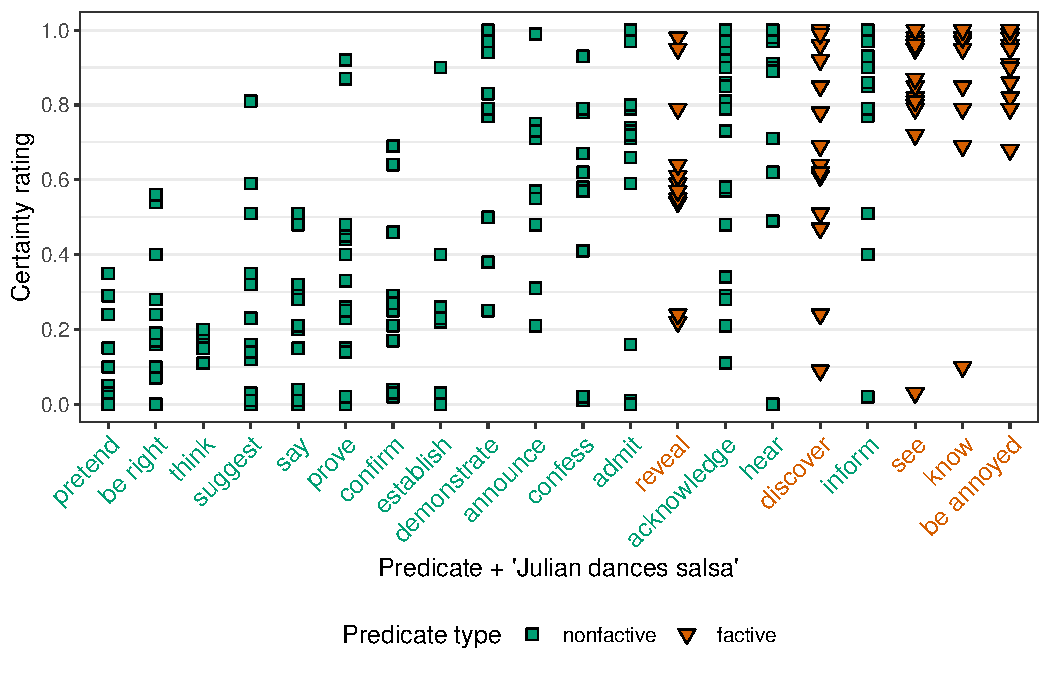
\includegraphics[width=.8\textwidth]{../../results/main/graphs/mean-certainty-by-predicateType-JULIAN}
%\caption{Participants' certainty ratings (measuring projection) of the CC that Julian dances salsa for the 20 \color{orange}factive \color{black} and \color{green}nonfactive \color{black} predicates investigated in Exp.~1a of \citealt{degen-tonhauser-language}.}\label{fig:dt1a-JULIAN}
%\end{figure}

\section{Conclusions}\label{s4}

For many decades the term `presupposition' has served researchers well to refer to content with properties distinct from, for instance, entailments, conventional implicatures and conversational implicatures. However, over the past two decades, both empirical and theoretical research has pointed out that the set of contents typically referred to as presuppositions is not as homogenous as perhaps initially assumed, resulting in theoretical analyses of particular subsets and an understanding of multiple dimensions of empirical variation among this set of contents. Against this background, the proposal by \citealt{mandelkern-etal2020} that there is an empirical measure that distinguishes presuppositions from nonpresuppositions sparked hope that there might be, after all, a way of preserving the term `presupposition' as a well-defined notion in the way it has been traditionally used.  Unfortunately, the results of our experiment did not support this claim. We suggest retiring the term `presupposition' or, at least, confining its use to a particular subtype of projective content, such as content associated with a strong contextual felicity constraint.

% end document here for word count
%\end{document}

\bibliographystyle{cslipubs-natbib}
%\bibliographystyle{/Users/tonhauser.1/Library/Latex/cslipubs-natbib}
\bibliography{bibliography}

\newpage

\section*{Supplemental materials}

\appendix

\setcounter{page}{1}
%\renewcommand{\thetable}{A\arabic{table}}

\setcounter{table}{0}
\renewcommand{\thetable}{A\arabic{table}}

\setcounter{figure}{0}
\renewcommand{\thefigure}{A\arabic{figure}}

\section{Experiment stimuli}\label{a:clauses}

The twenty clause-embedding predicates used in the experiment are the same as in \citealt{degen-tonhauser-openmind,degen-tonhauser-language}:

\begin{exe}
\ex\label{predicates}
\begin{xlist}
\ex Factive: be annoyed, discover, know, reveal, see
\ex Non-factive: acknowledge, admit, announce, be right, confess, confirm, establish, hear, inform, pretend, prove, say, suggest, think
\end{xlist}
\end{exe}
Eventive predicates, like {\em discover} and {\em hear}, were realized in the past tense and stative predicates, like {\em know} and {\em be annoyed}, were realized in the present tense. The direct object of {\em inform} was realized by the proper name {\em Sam}. Each clause-embedding predicate was paired with a unique subject proper name. The speaker of the target stimuli was realized by a randomly sampled unique proper name. 

The following list shows the 20 clauses that realized the complements of the predicates in the target stimuli, together with their lower and higher probability facts, respectively, that realized the preceding declarative sentences in the two support contexts.

\begin{enumerate}[leftmargin=4ex,itemsep=-2pt]
\item Mary is pregnant. Facts: Mary is a middle school student / Mary is taking a prenatal yoga class
\item Josie went on vacation to France. Facts:  Josie doesn't have a passport / Josie loves France 
\item Emma studied on Saturday morning. Facts: Emma is in first grade / Emma is in law school 
\item Olivia sleeps until noon. Facts: Olivia has two small children / Olivia works the third shift
\item Sophia got a tattoo. Facts: Sophia is a high end fashion model / Sophia is a hipster
\item Mia drank 2 cocktails last night. Facts: Mia is a nun / Mia is a college student
\item Isabella ate a steak on Sunday. Facts: Isabella is a vegetarian / Isabella is from Argentina
\item Emily bought a car yesterday. Facts: Emily never has any money / Emily has been saving for a year
\item Grace visited her sister. Facts: Grace hates her sister / Grace loves her sister
\item Zoe calculated the tip. Facts: Zoe is 5 years old / Zoe is a math major
\item Danny ate the last cupcake. Facts: Danny is a diabetic / Danny loves cake
\item Frank got a cat. Facts: Frank is allergic to cats / Frank has always wanted a pet
\item Jackson ran 10 miles. Facts: Jackson is obese / Jackson is training for a marathon
\item Jayden rented a car. Facts: Jayden doesn't have a driver's license / Jayden's car is in the shop
\item Tony had a drink last night. Facts: Tony has been sober for 20 years / Tony really likes to party with his friends
\item Josh learned to ride a bike yesterday. Facts: Josh is a 75-year old man / Josh is a 5-year old boy
\item Owen shoveled snow last winter. Facts: Owen lives in New Orleans / Owen lives in Chicago
\item Julian dances salsa. Facts: Julian is German / Julian is Cuban
\item Jon walks to work. Facts: Jon lives 10 miles away from work / Jon lives 2 blocks away from work
\item Charley speaks Spanish. Facts: Charley lives in Korea / Charley lives in Mexico
\end{enumerate}

\section{Filler and practice stimuli}\label{a:fillerPractice}

The following list shows the four filler stimuli where the interrogative was expected to receive high naturalness ratings in the context of the preceding declarative sentence. The values in parentheses indicate the mean naturalness rating that each of the four filler stimuli received. As shown, the third filler stimulus did not receive the expected high naturalness mean ratings, probably because participants were unwilling to accommodate that Hendrick has a car in a context in which Hendrick was looking to buy a car. This filler stimulus was therefore not used to exclude participants' data. 

\begin{enumerate}[leftmargin=4ex,itemsep=-2pt]

\item I don't know if Samantha has a new hat. Does Samantha have a new hat? (.89)

\item  I don't know if this pizza has mushrooms on it. Does this pizza have mushrooms on it? (.87)

\item Hendrick was looking to buy a car. Was Hendrick's car expensive? (.5)

\item Mary visited her aunt yesterday. Is Mary's aunt sick? (.91)

\end{enumerate}

\noindent
The following list shows the four practice stimuli in the order in which they were presented to the participants. Participants were able to advance to the experiment only if they gave a naturalness rating higher than .6 for the first and third stimulus, and a naturalness rating lower than .4 for the second and fourth stimulus.

\begin{enumerate}[leftmargin=4ex,itemsep=-2pt]

\item I have no idea where Natalie is from. Is Natalie from the USA?

\item I don't have any sisters. Have you met my sister yet?

\item I am going on vacation to Ireland. Does Fritz realize that Joe is going with me?

\item I have no idea if Anna has any dogs. Is Samuel glad that Anna fed her dogs?

\end{enumerate}

%\section{Model output: Pairwise comparison of expressions}\label{a:analysis1}
%
%{\bf JT PROPOSES TO LEAVE OUT THIS AND THE NEXT FIGURE}
%
%Fig.~\ref{fig:comparisons1} provides a graphical representation of the results of the pairwise comparisons between the ratings for each expression in the explicit ignorance context. The full model output in table form is available here: \url{LINK TO TABLE IN REPO}.
%
%\begin{sidewaysfigure}[h!]
%\centering
%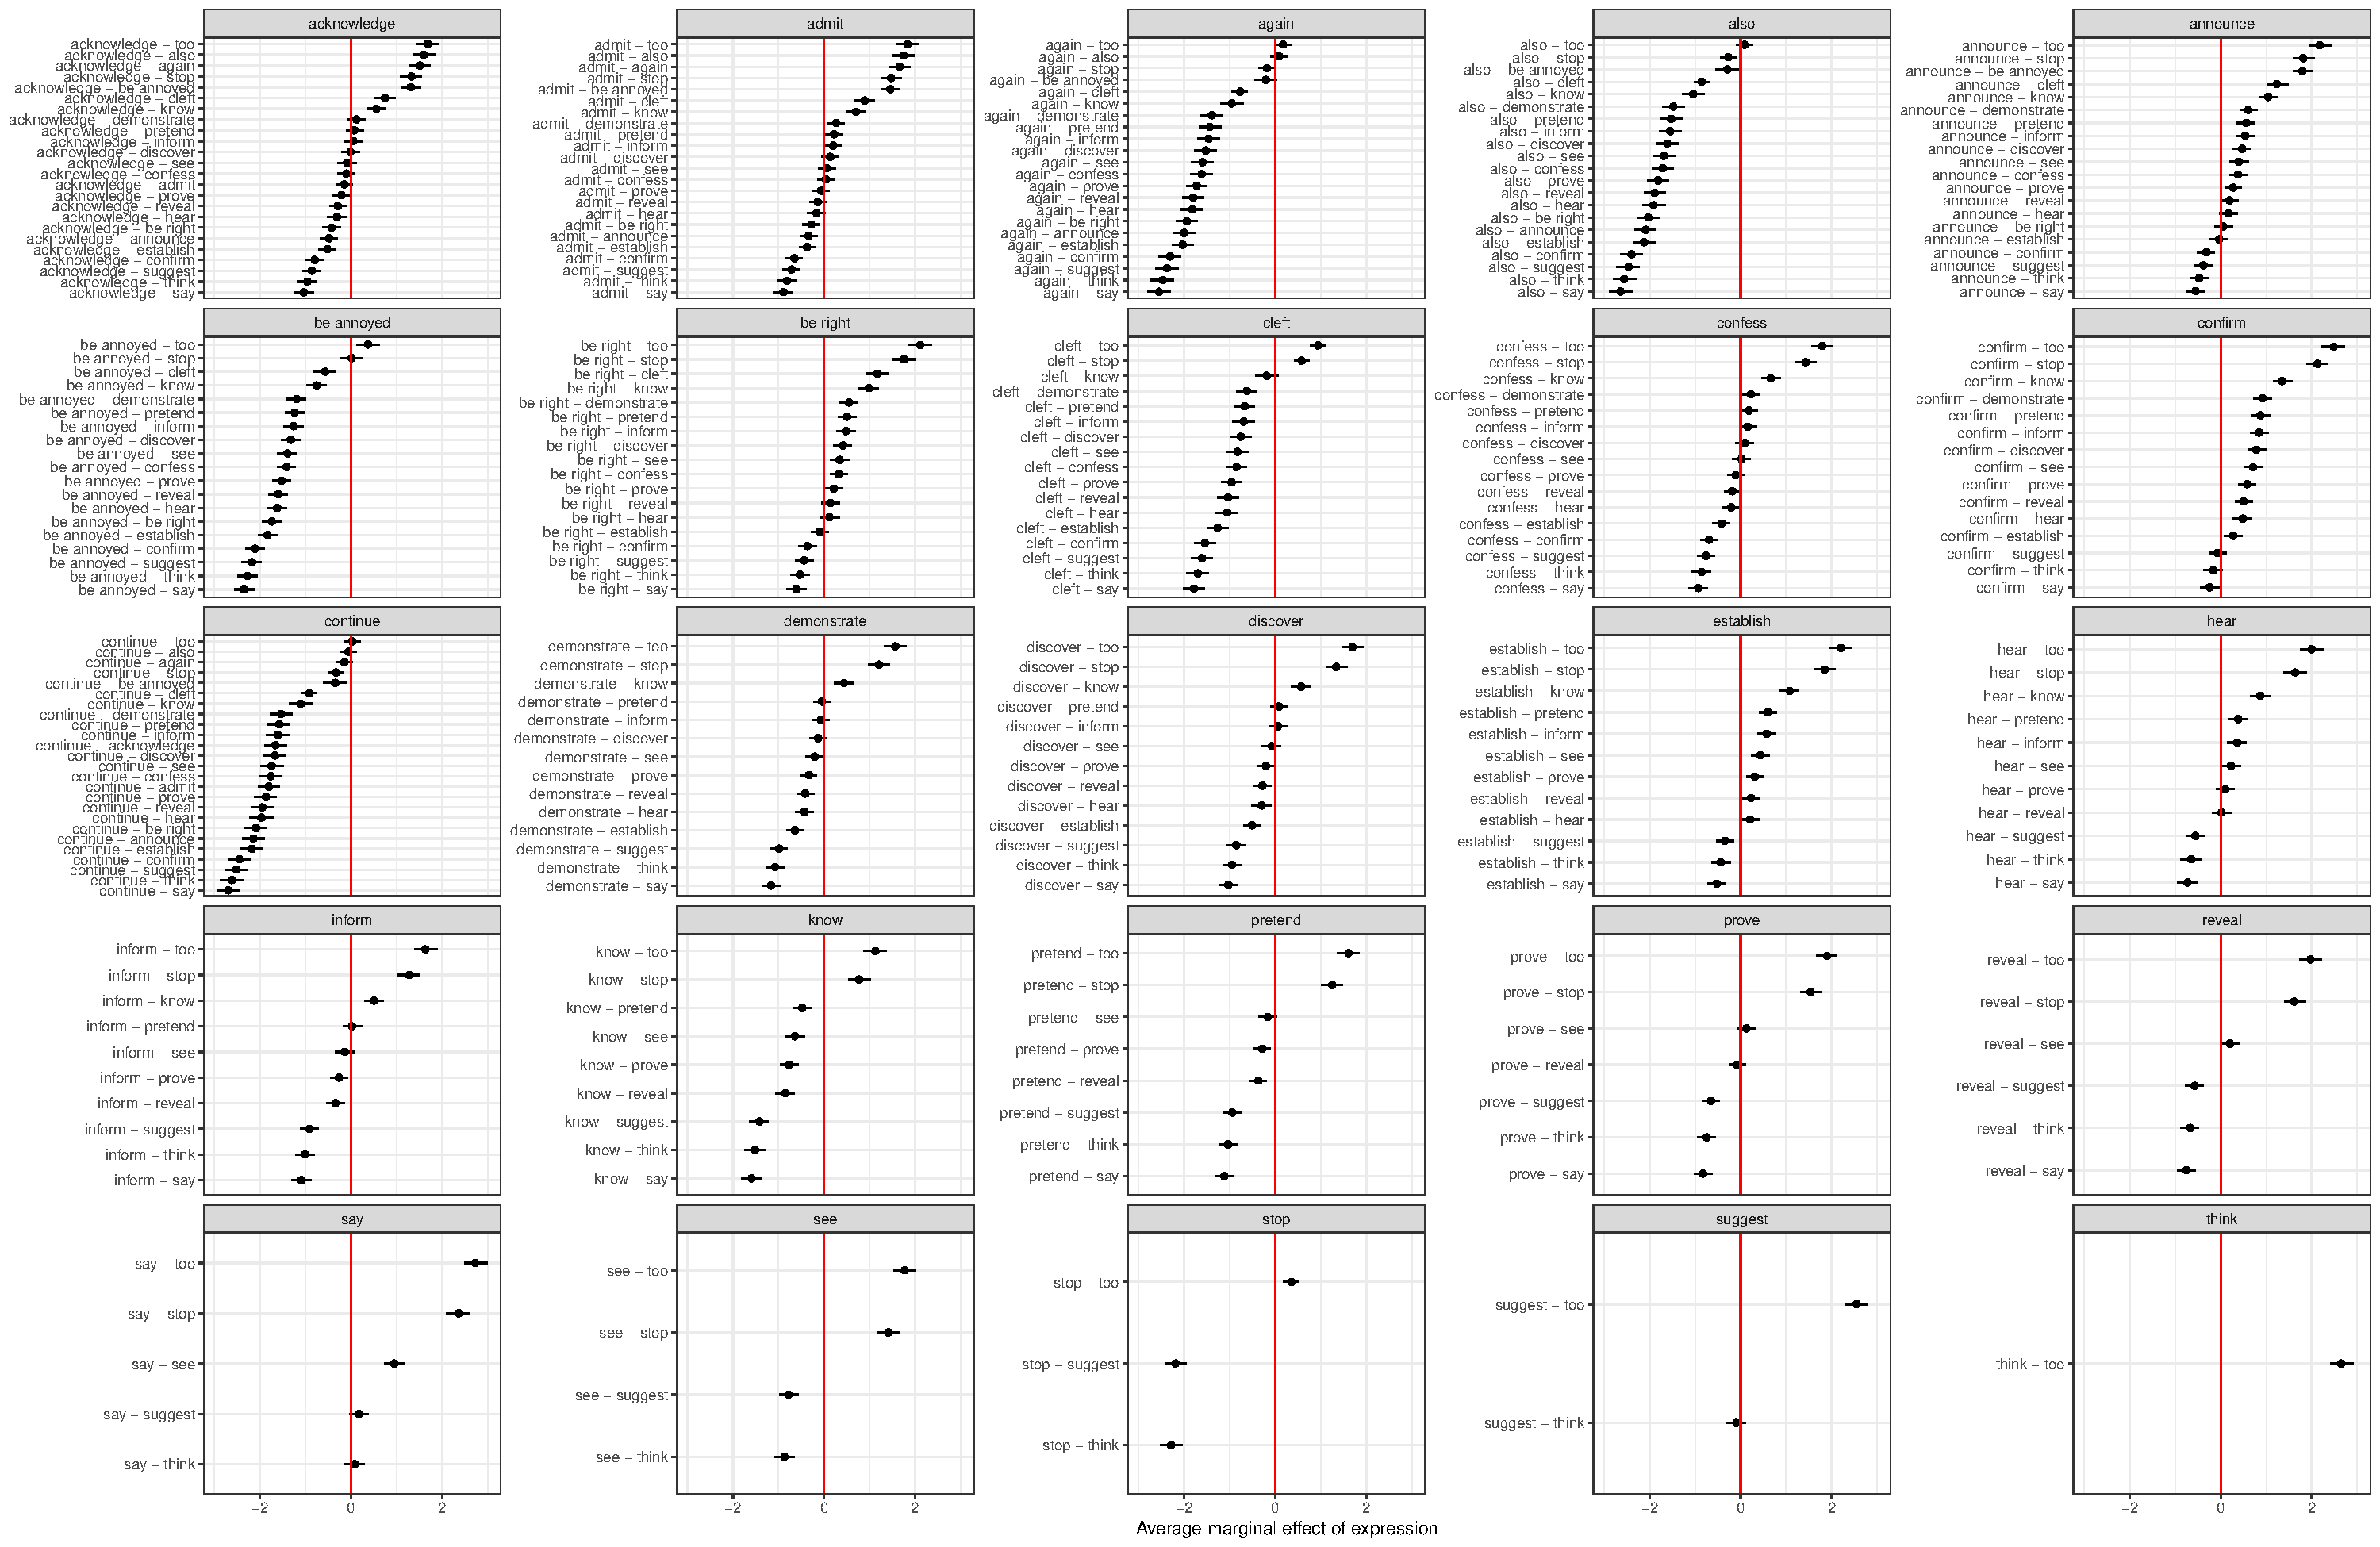
\includegraphics[width=\textwidth]{../../results/main/13explicitIgnorance/graphs/comparisons-in-EIC}
%\caption{.}\label{fig:comparisons1}
%\end{sidewaysfigure}
%
%\section{Model output: Pairwise comparison of contexts}\label{a:analysis2}
%
%Fig.~\ref{fig:comparisons2} provides a graphical representation of the results of the pairwise comparisons of the ratings in the three contexts for each of the 20 predicates. The full model output in table form is available here: \url{LINK TO TABLE IN REPO}.
%
%\begin{figure}[h!]
%\centering
%\includegraphics[width=.8\textwidth]{../../results/main/13explicitIgnorance/graphs/context-comparisons}
%\caption{.}\label{fig:comparisons2}
%\end{figure}
 
\end{document}

